\documentclass[12pt]{article}

\usepackage[utf8]{inputenc}
\usepackage[T1]{fontenc}
\usepackage{mwe}
\usepackage{graphicx}
\usepackage{epsfig}
\usepackage{cite}
\usepackage{geometry}
\usepackage{float}
\usepackage{subfig}
\usepackage{comment}
\usepackage{listings}
\usepackage{xcolor}
\usepackage{pdfpages}

\lstset{upquote=true,columns=fullflexible,literate={*}{{\char42}}1{-}{{\char45}}1}

\title{Two Way Switch}

\maketitle
\begin{figure}[!htb]
\centering
  
\includegraphics[width=3cm,keepaspectratio]{logo.png}\textbf{ }\textbf{  }
  
\includegraphics[width=3cm,keepaspectratio]{download.png}\textbf{  }
  
\includegraphics[width=3cm,keepaspectratio]{modelsim-logo.jpg}
\end{figure}	
	\begin{minipage}{0.4\textwidth}
		\begin{flushleft} \large
			\emph{Mentors}\\
			Prasad T\\
            Aditya Gudla\\
            Simranjeet Singh \
			\end{flushleft}
			\end{minipage}~
			\begin{minipage}{0.4\textwidth}
            
			\begin{flushright} \large
			\emph{Interns} \\
			Ajay Chaudhari\\
            Chethan T Bhat\\
            Ritvik Tiwari \\
            Karthik A Shet \\
		\end{flushright}
	\end{minipage}\\[2 cm]
\begin{document}



\newpage
\tableofcontents
\newpage
\section{Introduction}

\subsection{What is a Two Way Switch ?}
A two way switch can be explained using a simple example. Consider a room with two switches and one bulb. Now, If both the switches are in OFF state or ON state the bulb will not glow. But, If either of the two switch is ON the bulb will glow. If we have to relate this with digital electronics, the logic can be realised using an X-OR gate.

\subsection{X-OR Gate}
XOR gate (pronounced as Exclusive OR) is a digital logic gate that gives a \textbf{TRUE} (1 or HIGH) output when odd number of inputs are \textbf{TRUE}. 

\begin{figure}[H]
    \centering
    \begin{minipage}{0.45\textwidth}
        \centering
        
\includegraphics[width=0.9\textwidth]{img1} 
        \caption{Logic Symbol}
    \end{minipage}\hfill
    \begin{minipage}{0.45\textwidth}
        \centering
        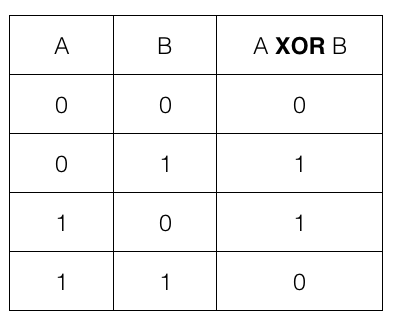
\includegraphics[width=0.9\textwidth]{img2} 
        \caption{Truth Table}
    \end{minipage}
\end{figure}

\newpage
\section{Circuit Diagram}
\textbf{Note:} LED does not conduct in both direction. This circuit is just a representation of the logic
\begin{figure}[H]
    \centering
    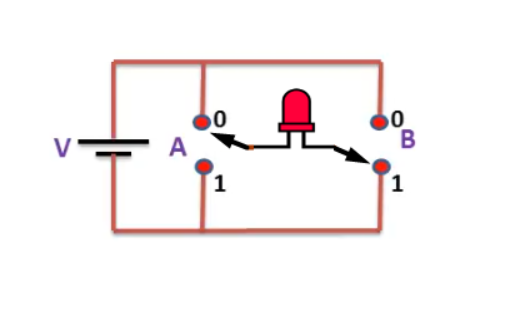
\includegraphics[scale=1.2]{new circuit.png}
    \caption{Two way switch Circuit Diagram.}
\end{figure}

\section{Code in VHDL \& Verilog}
\subsection{Verilog Code(RTL Description)}

\noindent Dataflow Modelling:
\definecolor{vgreen}{RGB}{104,180,104}
\definecolor{vblue}{RGB}{49,49,255}
\definecolor{vorange}{RGB}{255,143,102}


\lstdefinestyle{verilog-style}
{
    language=Verilog,
    frame=single,
    column=fullflexible,
    basicstyle=\small\ttfamily,
    keywordstyle=\color{vblue},
    identifierstyle=\color{black},
    commentstyle=\color{vgreen},
    moredelim=*[s][\colorIndex]{[}{]},
    literate=*{:}{:}1
}

\makeatletter
\newcommand*\@lbracket{[}
\newcommand*\@rbracket{]}
\newcommand*\@colon{:}
\newcommand*\colorIndex{%
    \edef\@temp{\the\lst@token}%
    \ifx\@temp\@lbracket \color{black}%
    \else\ifx\@temp\@rbracket \color{black}%
    \else\ifx\@temp\@colon \color{black}%
    \else \color{vorange}%
    \fi\fi\fi
}
\makeatother

\begin{lstlisting}[style =verilog-style]
//Verilog code in Dataflow style

module TWS(
	input s1,s2,	//Define two Inputs pins
	output z);	//Define one output pin
	assign z = (s1^s2);  //XOR the 2 input pins(s1,s2) and assign  
	                   //the output to the output pin(X1)
endmodule

\end{lstlisting}
\newpage
\noindent Behavioural Modelling:
\begin{lstlisting}[style = verilog-style]
//Verilog code in Behavioural style
module TWS(
	input s1,s2,   	 //Define two inputs(switches)
	output reg z	 //Define the output pin
	);
	
always @ (s1,s2)    //Every time the input changes, the output
		  //is to be updated
begin
	if (s1==s2) //if both switches are in same position, 
	            //output is LOW
		z = 0;
	else
		z=1;	//if the position of switches are not equal, 
		        //output is HIGH
end
endmodule

\end{lstlisting}

\subsection{Testbench Code(Verilog)}
\begin{lstlisting}[style=verilog-style]
module TWS_tb;
reg s1;reg s2; //define input
wire z;       //define output

TWS uut(.s1(s1),.s2(s2),.z(z)); //Map testbench ports with 
                                                //DUT ports

initial begin
	s1 = 0; s2 = 0;#100;  //different combinations of input
	s1 = 0; s2 = 1;#100;
	s1 = 1; s2 = 0;#100;
	s1 = 1; s2 = 1;#100;
	#100;
end
endmodule 
\end{lstlisting}
\newpage
\subsection{VHDL Code(RTL Description)}
\noindent Dataflow Modelling:
\definecolor{vgreen}{RGB}{104,180,104}
\definecolor{vblue}{RGB}{49,49,255}
\definecolor{vorange}{RGB}{255,143,102}


\lstdefinestyle{vhdl-style}
{
    language=VHDL,
    frame=single,
    linewidth=17cm,
    basicstyle=\small\ttfamily,
    keywordstyle=\color{vblue},
    identifierstyle=\color{black},
    commentstyle=\color{vgreen},
    moredelim=*[s][\colorIndex]{[}{]},
    literate=*{:}{:}1
}

\makeatletter
\newcommand*\@lbracket{[}
\newcommand*\@rbracket{]}
\newcommand*\@colon{:}
\newcommand*\colorIndex{%
    \edef\@temp{\the\lst@token}%
    \ifx\@temp\@lbracket \color{black}%
    \else\ifx\@temp\@rbracket \color{black}%
    \else\ifx\@temp\@colon \color{black}%
    \else \color{vorange}%
    \fi\fi\fi
}
\makeatother
\begin{lstlisting}[style=vhdl-style]
LIBRARY IEEE;
USE IEEE.STD_LOGIC_1164.ALL;

ENTITY Two_Way_Switch is
	PORT(
		A		: IN STD_LOGIC ;	--Switch 1	
		B		: IN STD_LOGIC ;	--Switch 2
		C 		: OUT STD_LOGIC		--LED Output
	);
END Two_Way_Switch;
ARCHITECTURE DATAFLOW OF Two_Way_Switch IS
BEGIN
	C <= A XOR B;					-- XOR logic used for two way switch
END DATAFLOW;


\end{lstlisting}
%\newpage
\noindent Behavioural Modelling:

\begin{lstlisting}[style=vhdl-style]
LIBRARY IEEE;
USE IEEE.STD_LOGIC_1164.ALL;

ENTITY Two_Way_Switch_Behavioural IS
PORT ( 
	A :IN STD_LOGIC; -- SWITCH 1
	B :IN STD_LOGIC; -- SWITCH 2
	C :OUT STD_LOGIC -- LED OUTPUT
);
END Two_Way_Switch_Behavioural;
ARCHITECTURE BEHAVIORAL OF Two_Way_Switch IS
	BEGIN
		PROCESS (A, B) 		--USED FOR BEHAVIORAL MODELLING
			BEGIN
			IF (A/=B) THEN 	--IF EITHER ONE OF THE SWITCHES IS ON
			C <= '1'; 		--LED WILL GLOW
			ELSE 			--IF BOTH THE SWITCHES ARE ON OR OFF
			C <= '0'; 		--LED WILL NOT GLOW
		END IF;
	END PROCESS;
END BEHAVIORAL;
\end{lstlisting}

\subsection{Testbench Code(VHDL)}
\begin{lstlisting}[style= vhdl-style]
LIBRARY IEEE;
USE IEEE.STD_LOGIC_1164.ALL;

ENTITY Two_Way_Switch_TB IS					--defining the entity
END Two_Way_Switch_TB;

ARCHITECTURE BEHAVIOR OF Two_Way_Switch_TB IS	--defining the architecture
COMPONENT Two_Way_Switch						--two way switch design
	PORT(
		A		: IN STD_LOGIC ;				--Switch 1
		B		: IN STD_LOGIC;					--Switch 2
		C 		: OUT STD_LOGIC					--LED Output
	);
END COMPONENT;
	
	SIGNAL A 	: STD_LOGIC := '0';				--Stimulus signal for switch 1
	SIGNAL B	: STD_LOGIC := '0';				--Stimulus signal for switch 2
	SIGNAL C 	: STD_LOGIC := '0';				--Output signal
			
	BEGIN
	--defining unit under test i.e
	--two way switch
	UUT : Two_Way_Switch PORT MAP (A => A ,B=> B, C=> C);
	
	--begining stimulation process
	StimulusProcess : PROCESS
	BEGIN
		A <= '0';
		B <= '0';
		WAIT FOR 100 NS;
		
		A <= '1';
		B <= '0';
		WAIT FOR 100 NS;

		A <= '0';
		B <= '1';
		WAIT FOR 100 NS;
		
		A <= '1';
		B <= '1';
		WAIT FOR 100 NS;
		WAIT ;
	END PROCESS;
END BEHAVIOR;
\end{lstlisting}
\newpage

\section{Implementing on quartus II}
 To Implement the design in Quartus Software, follow these steps(For more detailed information on the following steps, refer 'Quick Start Guide to Quartus and ModelSim Software' Document):

\noindent \textbf{Note:} For this demonstration, the language used is Verilog HDL. Device is DE0-Nano FPGA Board.\newline
\hspace*{35pt}\textbf{Family:}Cyclone IV E; \textbf{Chip Name:}EP4CE22F17C6
\begin{enumerate}
    \item Start a new project in Quartus Lite software
    \begin{figure}[H]
    \centering
    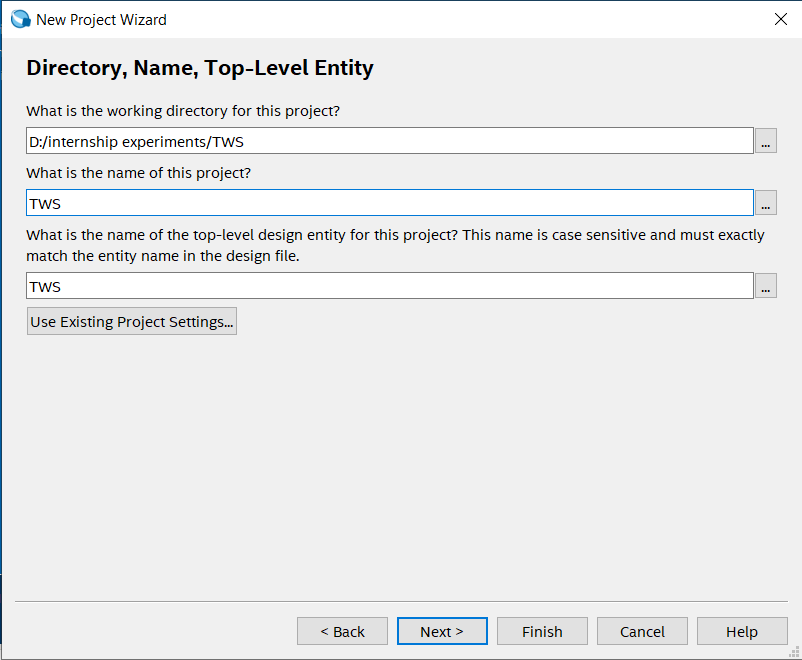
\includegraphics[width=13cm,keepaspectratio]{TWS new1.png}
    \end{figure}
    \newpage
    \item Create a new Verilog or VHDL file.Here we create a Verilog file for demonstration.Same procedure can be followed to VHDL file.
    
    \begin{figure}[H]
        \centering
    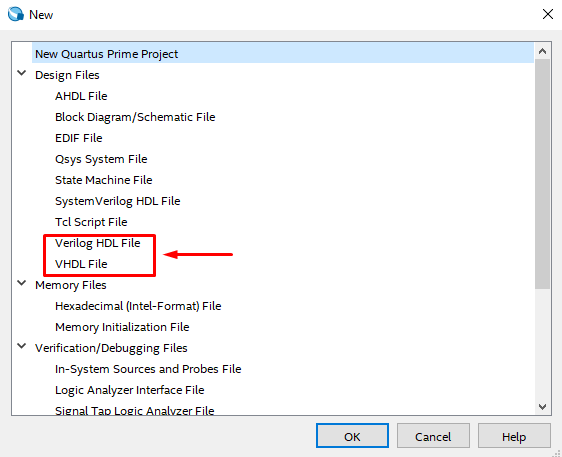
\includegraphics[width=8cm,keepaspectratio]{Implement on Quartus/img2.png}
    \end{figure}
    \item Type the above main code in this file and make sure than the Module name and the file name is same.\newline \textbf{Note:}We have used the Dataflow Verilog code for this demonstration 
    \begin{figure}[H]
        \centering
    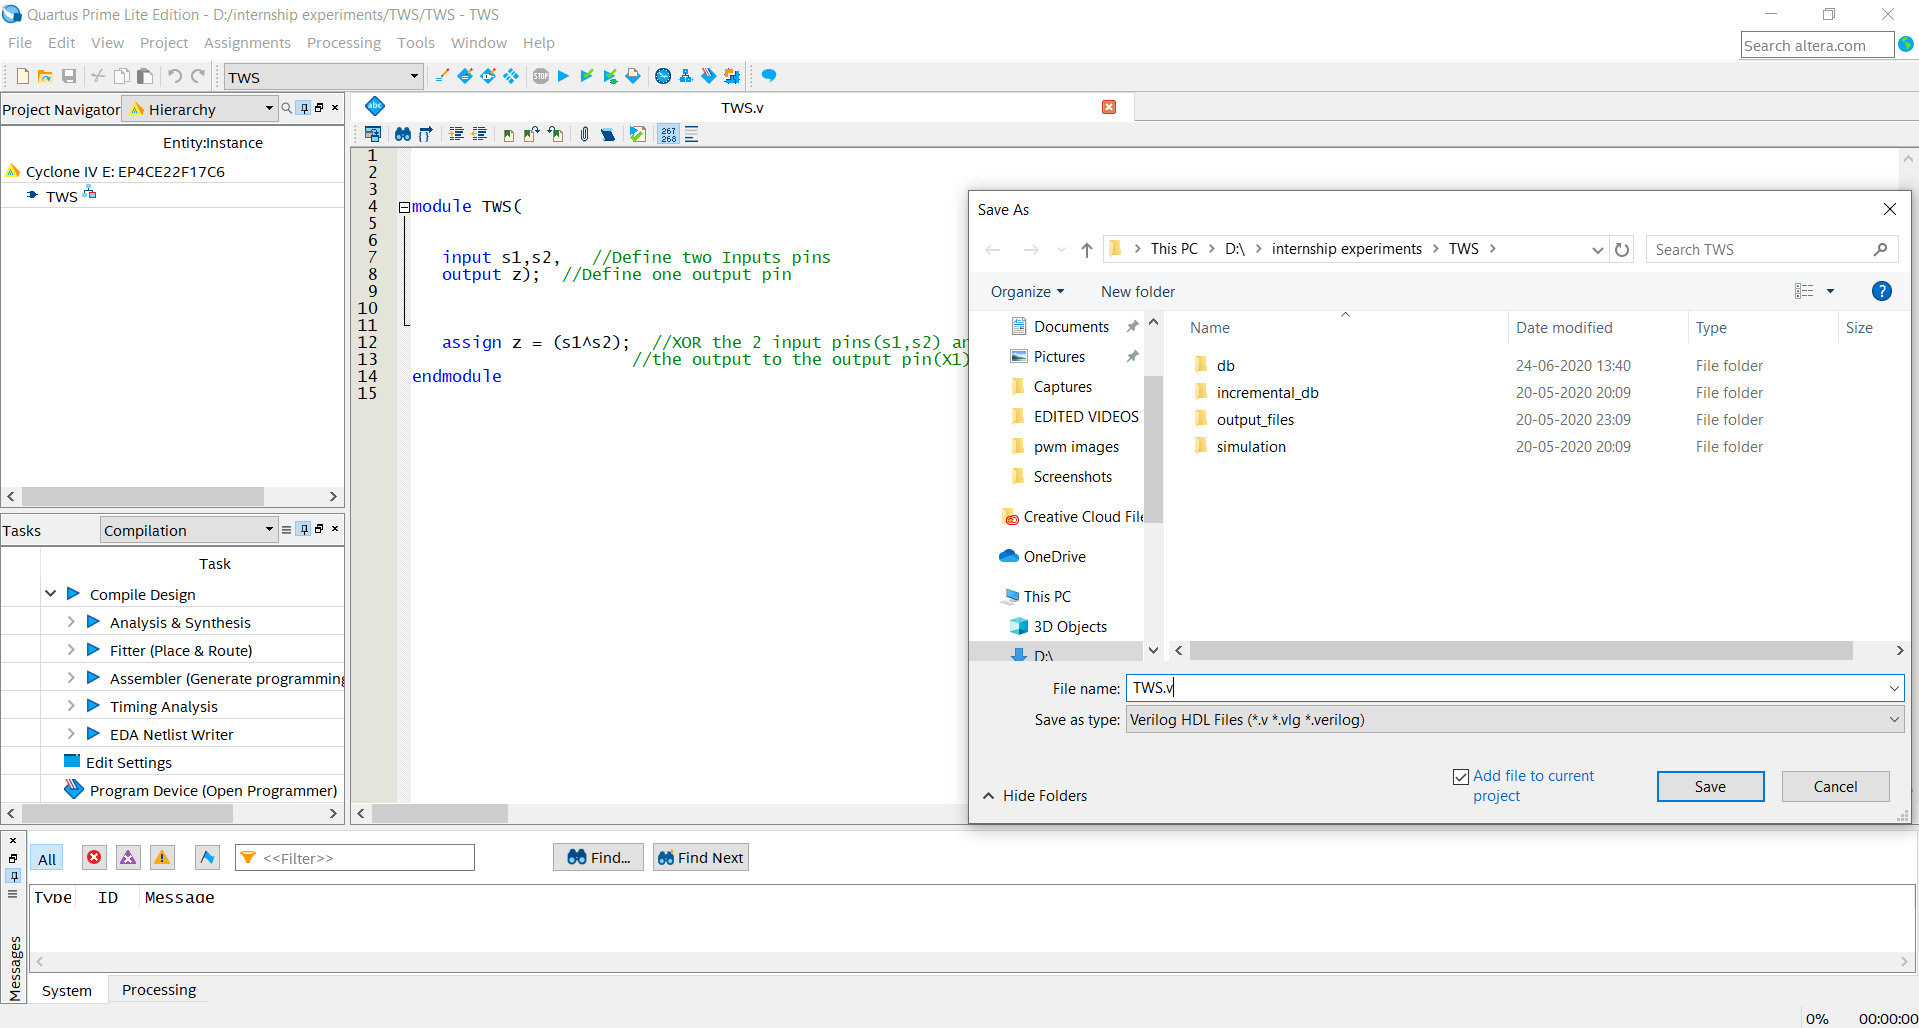
\includegraphics[width=14cm,keepaspectratio]{twsnew3.png}
    \end{figure}
    \newpage
    \item Go to \textbf{'Project' $\rightarrow$  'Set as Top-Level Entity'}.
    \begin{figure}[H]
        \centering
    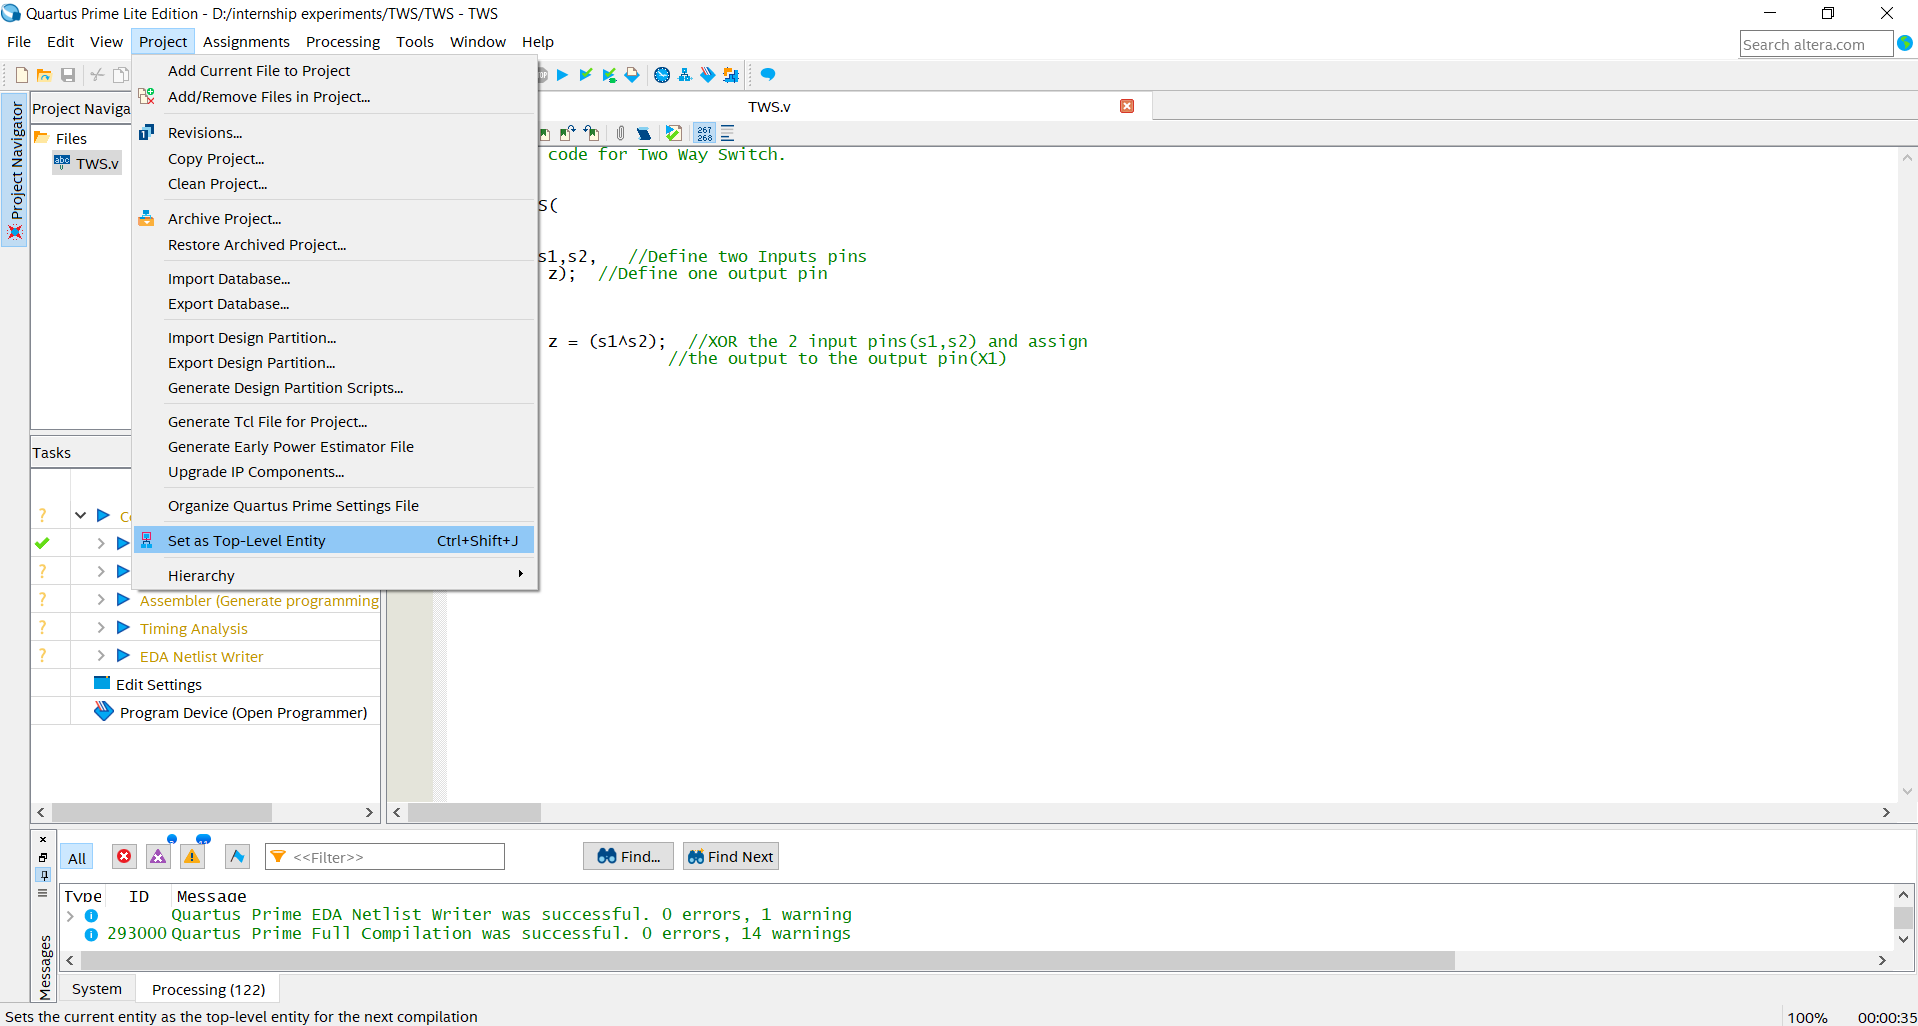
\includegraphics[width=14cm,keepaspectratio]{SETAS.png}
    \end{figure}
    
    \item Go to \textbf{'Processing'  $\rightarrow$ 'Start Compilation'}.
    \begin{figure}[H]
        \centering
    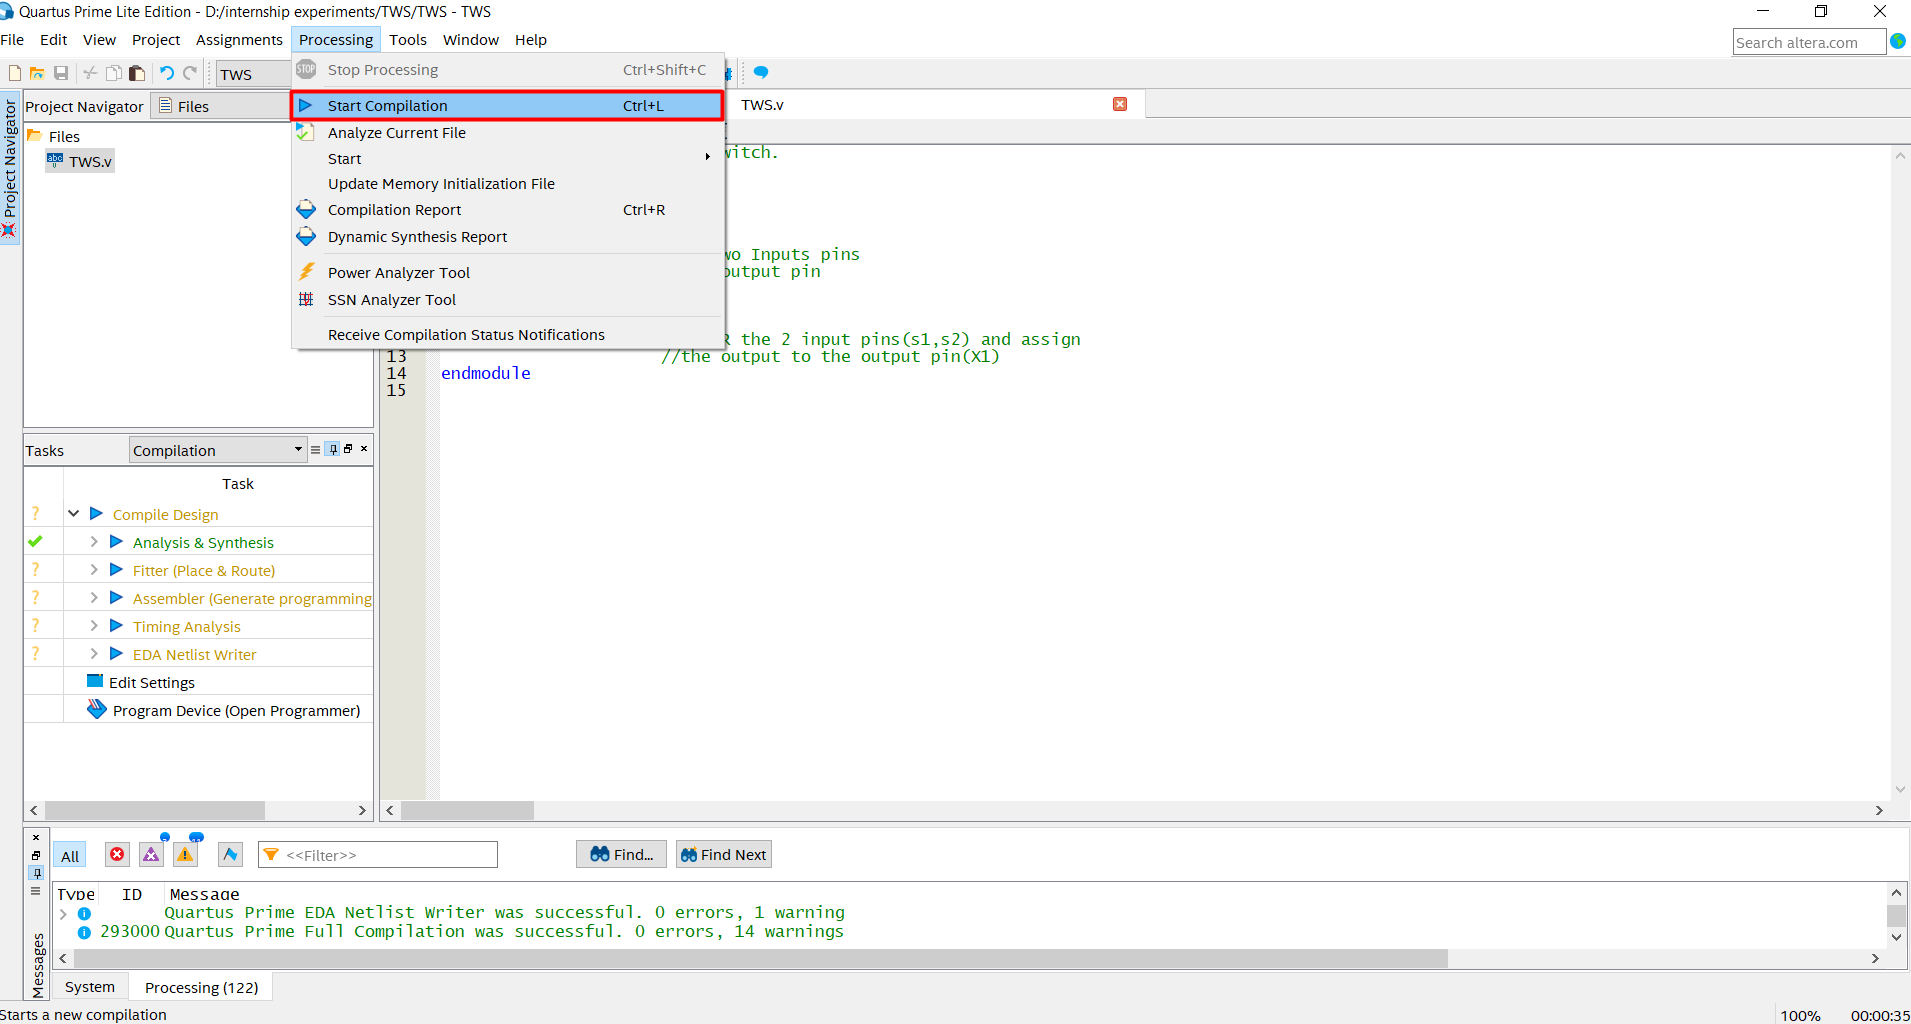
\includegraphics[width=14cm,keepaspectratio]{TWSCOM.png}
    \end{figure}
    
    \newpage
    
    \item After successful compilation, you will see these \textcolor{green}{Green} check marks.
    \begin{figure}[H]
        \centering
    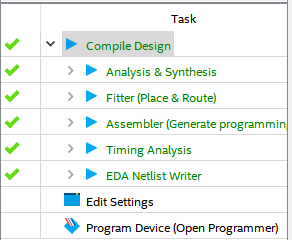
\includegraphics[keepaspectratio]{check_marks.png}
    \end{figure}
\end{enumerate}

\newpage

\section{RTL Circuit of the implemented design}
The below two figures show the RTL Circuit of the two different type of modelling (Dataflow and behavioural). As it can be seen , both types of modelling resulted in the same type of design. Although this is not possible for more complex designs(Behavioural modelling results in a more complex circuit than Dataflow or Structural), intelligent and smart behavioural design can lead to really well optimised circuits.\vspace{1cm}
\\\
    \textbf{Steps to get RTL circuit.}
    \vspace{4mm}
        \begin{enumerate}
            \item Go to \textbf{'Tools' $\rightarrow$  'Netlist Viewers' $\rightarrow$ 'RTL Viewer'}.
            \vspace{6mm}
                \begin{figure}[H]
                     \centering
                    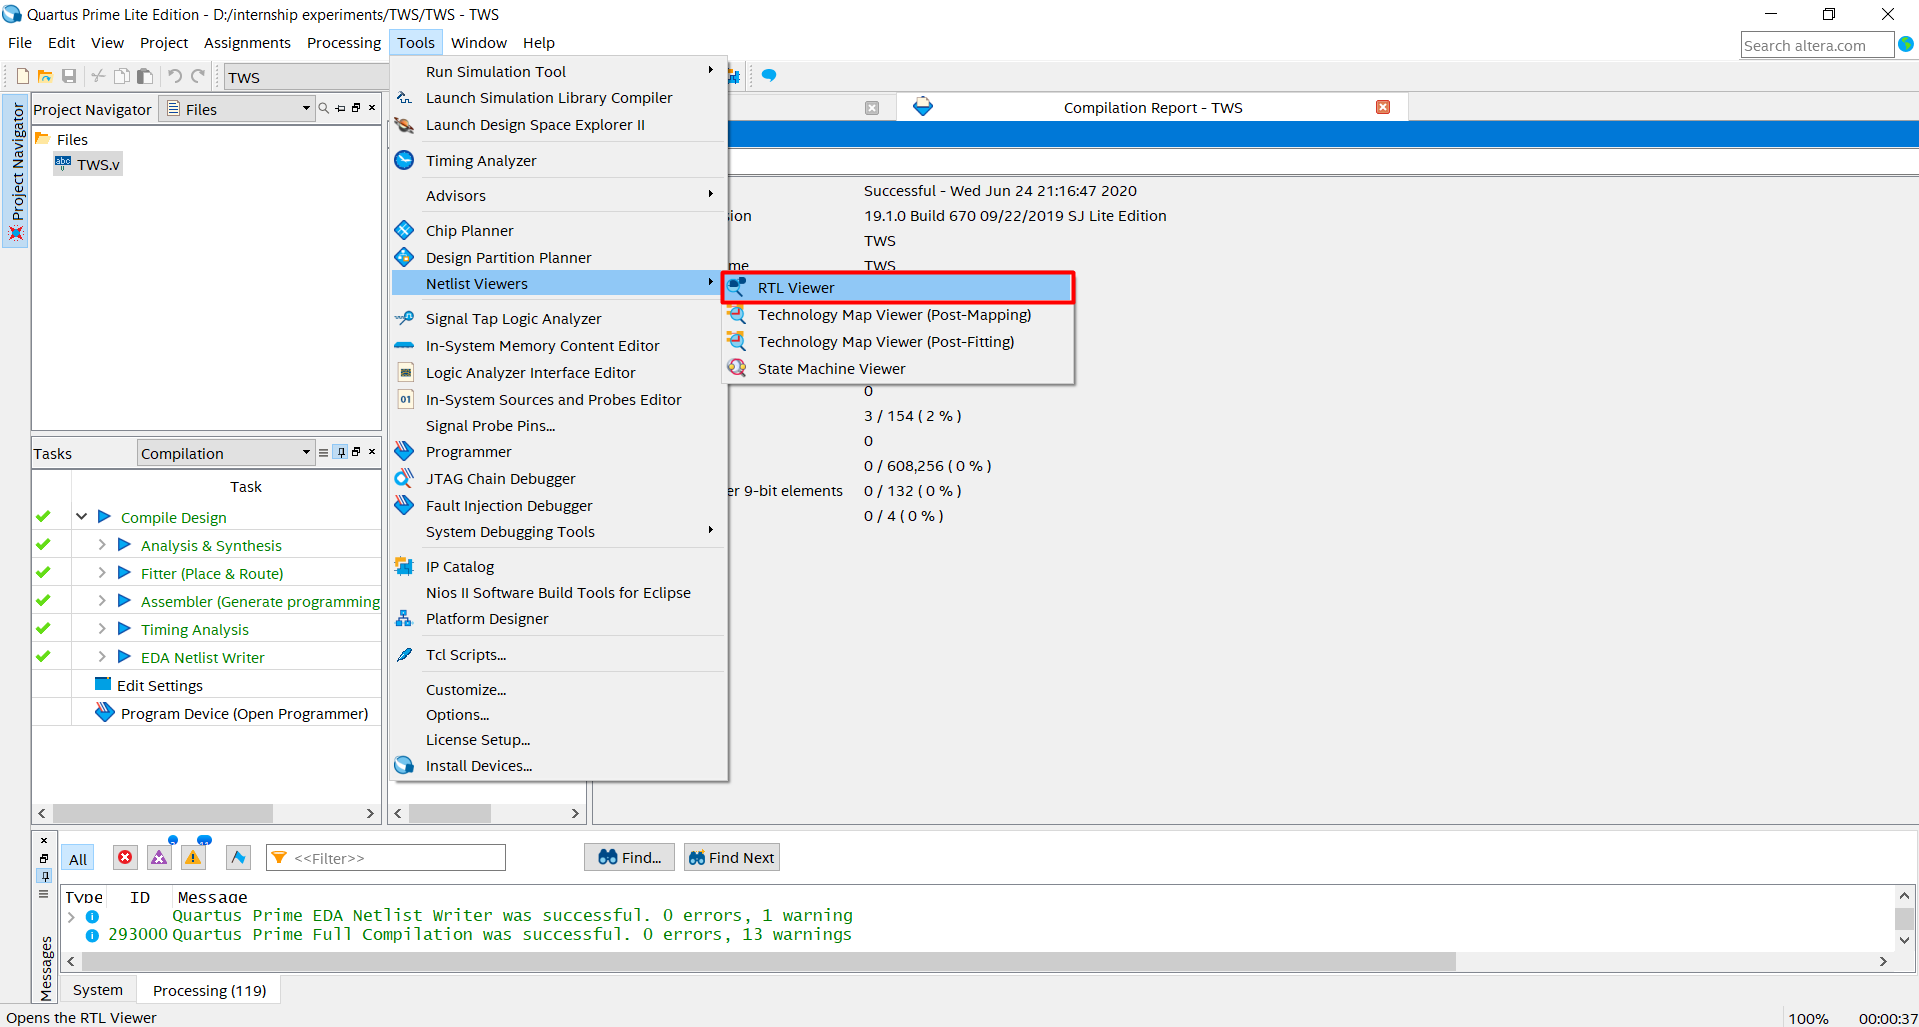
\includegraphics[scale=0.35]{TWSRTL1.png}
                \end{figure}
                \newpage
            \item The below figure shows the equivalent RTL circuit in both Dataflow and Behavioural modelling styles.      
\begin{figure}[H]
    \centering
    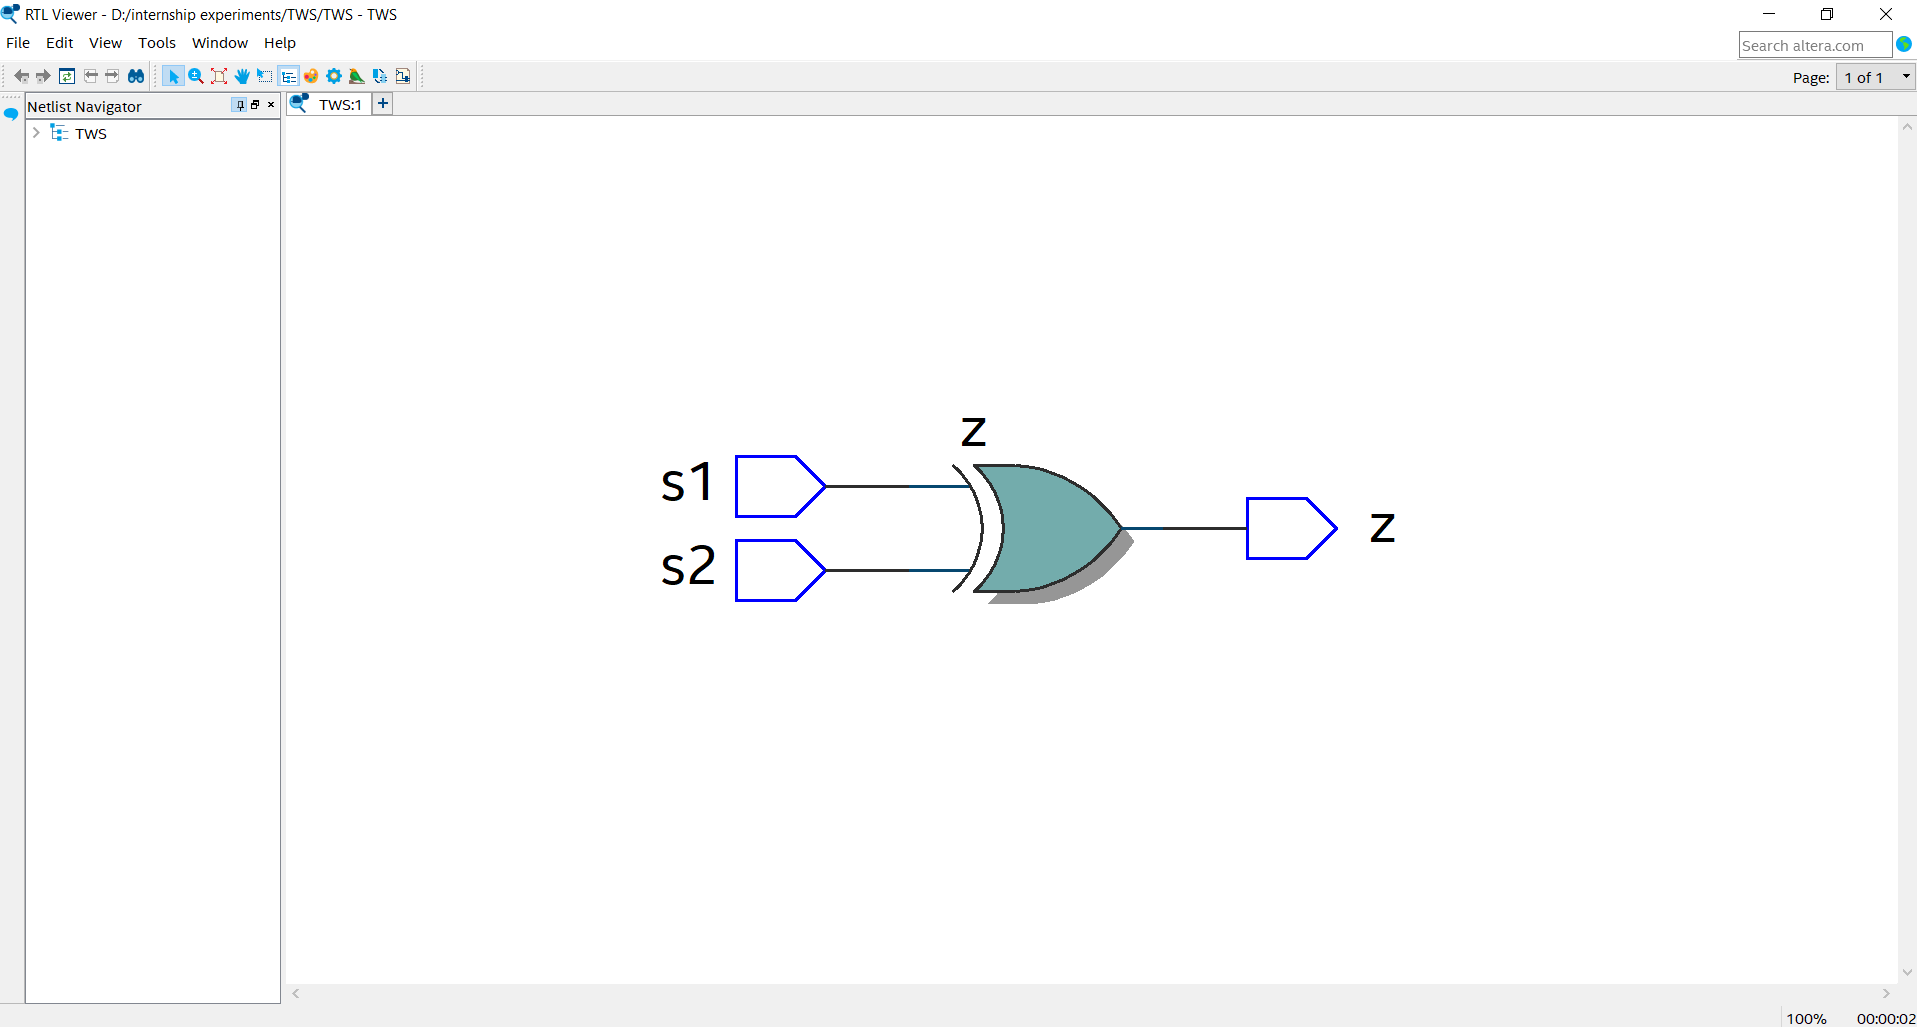
\includegraphics[scale=0.35]{TWSRTL2.png}
    \caption{Dataflow modelling}
\end{figure}
\begin{figure}[H]
    \centering
    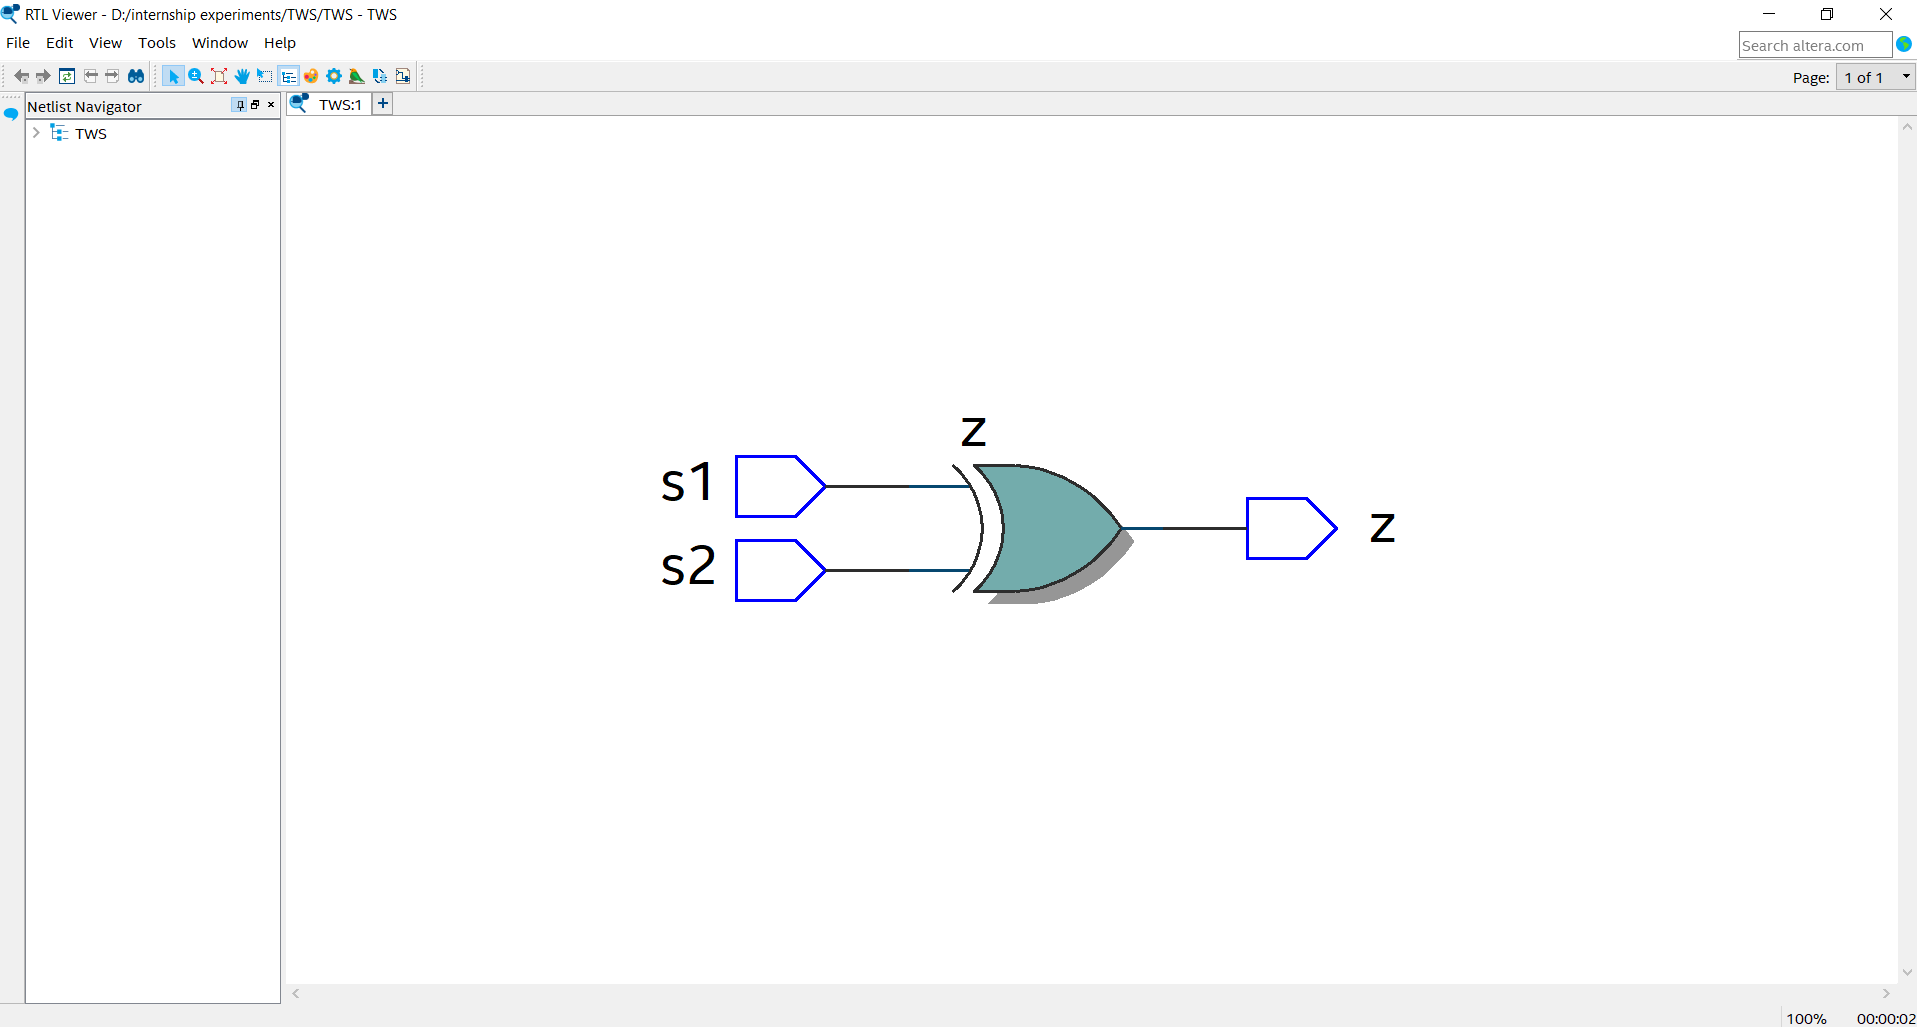
\includegraphics[scale=0.35]{TWSRTL2.png}
    \caption{Behavioural modelling}
\end{figure}
\end{enumerate}

\section{Pin  Assignment}
\begin{enumerate}
    \item Click on \textbf{'Assignments' $\rightarrow$ 'Pin Planner'},This Pin Planner shows the I/O ports that we have created in our design.
    \begin{figure}[H]
        \centering
        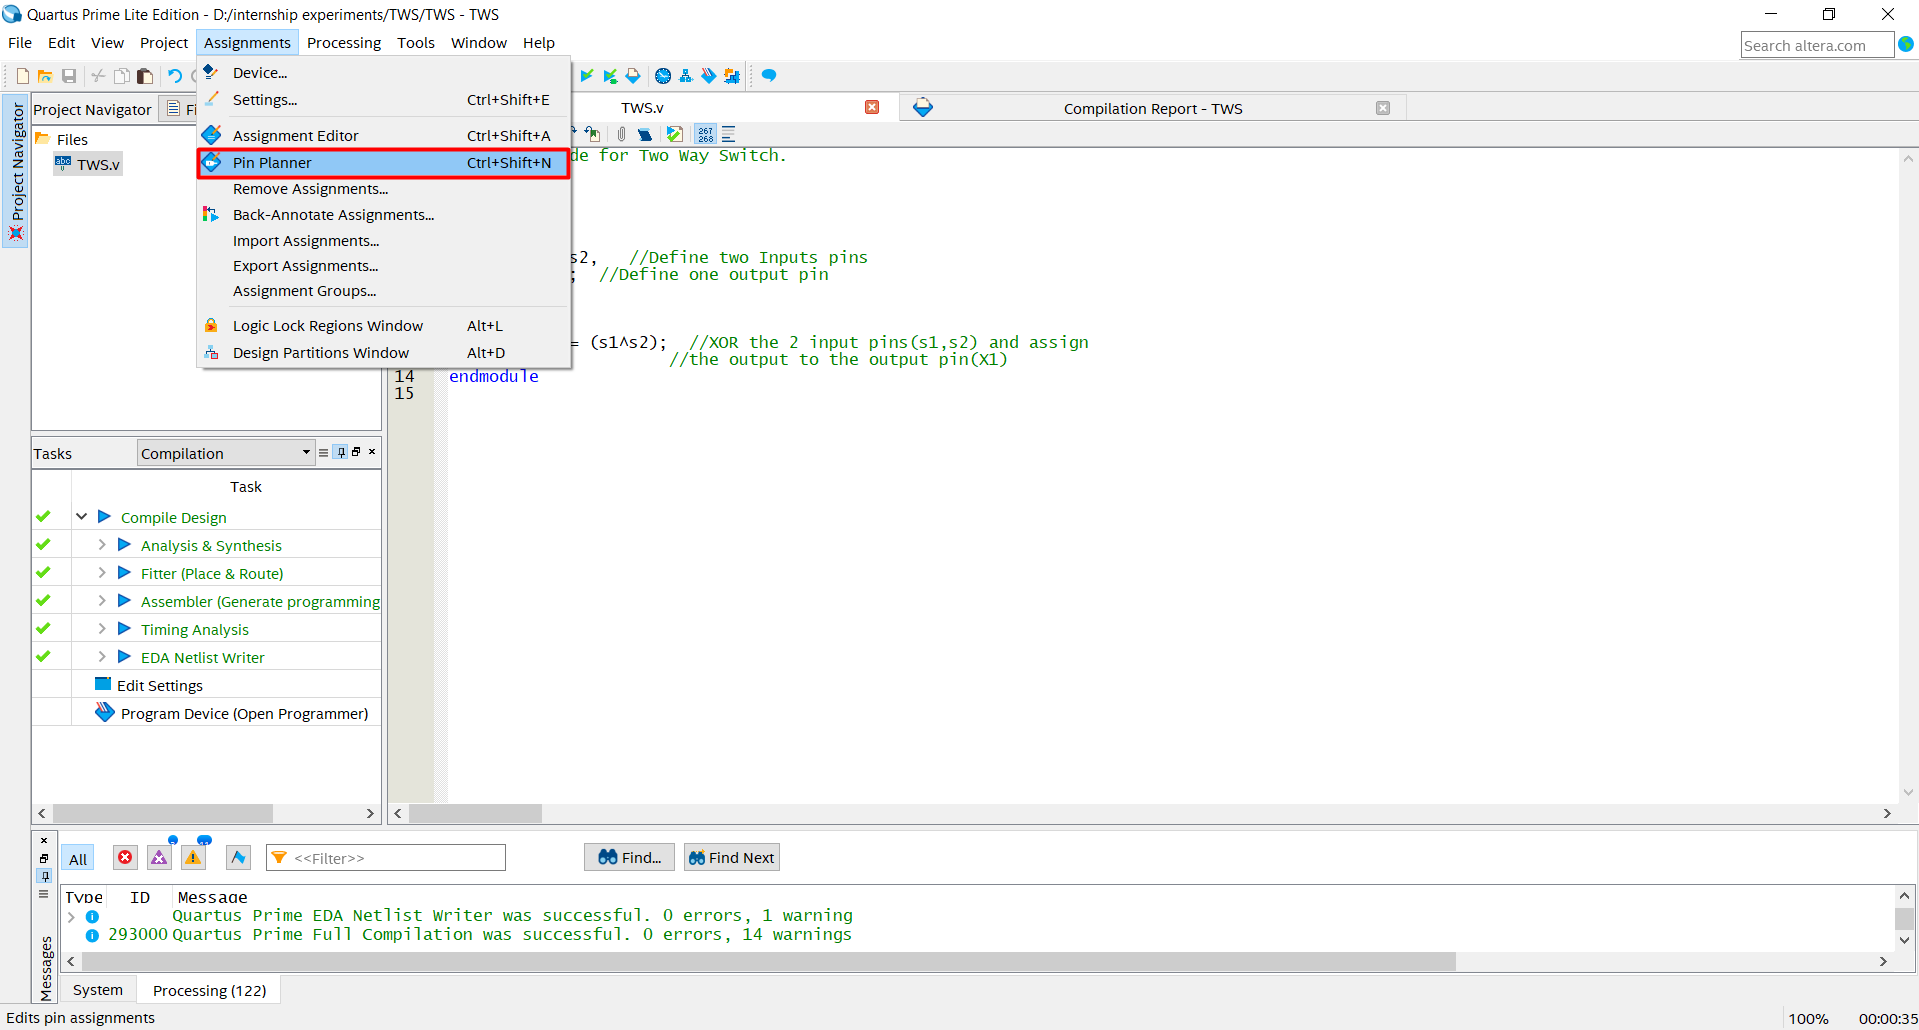
\includegraphics[scale=0.35]{twsplan1.png}
    \end{figure}

    \item Now we have to assign each I/O ports with the respective Pin numbers, which can be found on the Device Manual of the FPGA Board.Here we are Referring to the DEO NANO Board user manual .Out of 8 LED present in the DEO NANO Board We will select \textbf{LED[0]} as the output 'z' of the XOR gate ,whose PIN number is \textbf{PIN\_A15}. And out of 4 DIP Switches present in DEO NANO Board we use two DIP switches \textbf{DIP\_SWITCH[0]} and \textbf{DIP\_SWITCH[1]} for input signal 'S1' and 'S2',whose PIN numbers are \textbf{PIN\_M1} and \textbf{PIN\_T8} respectively.
    \newpage
     \begin{figure}[H]
        \centering
        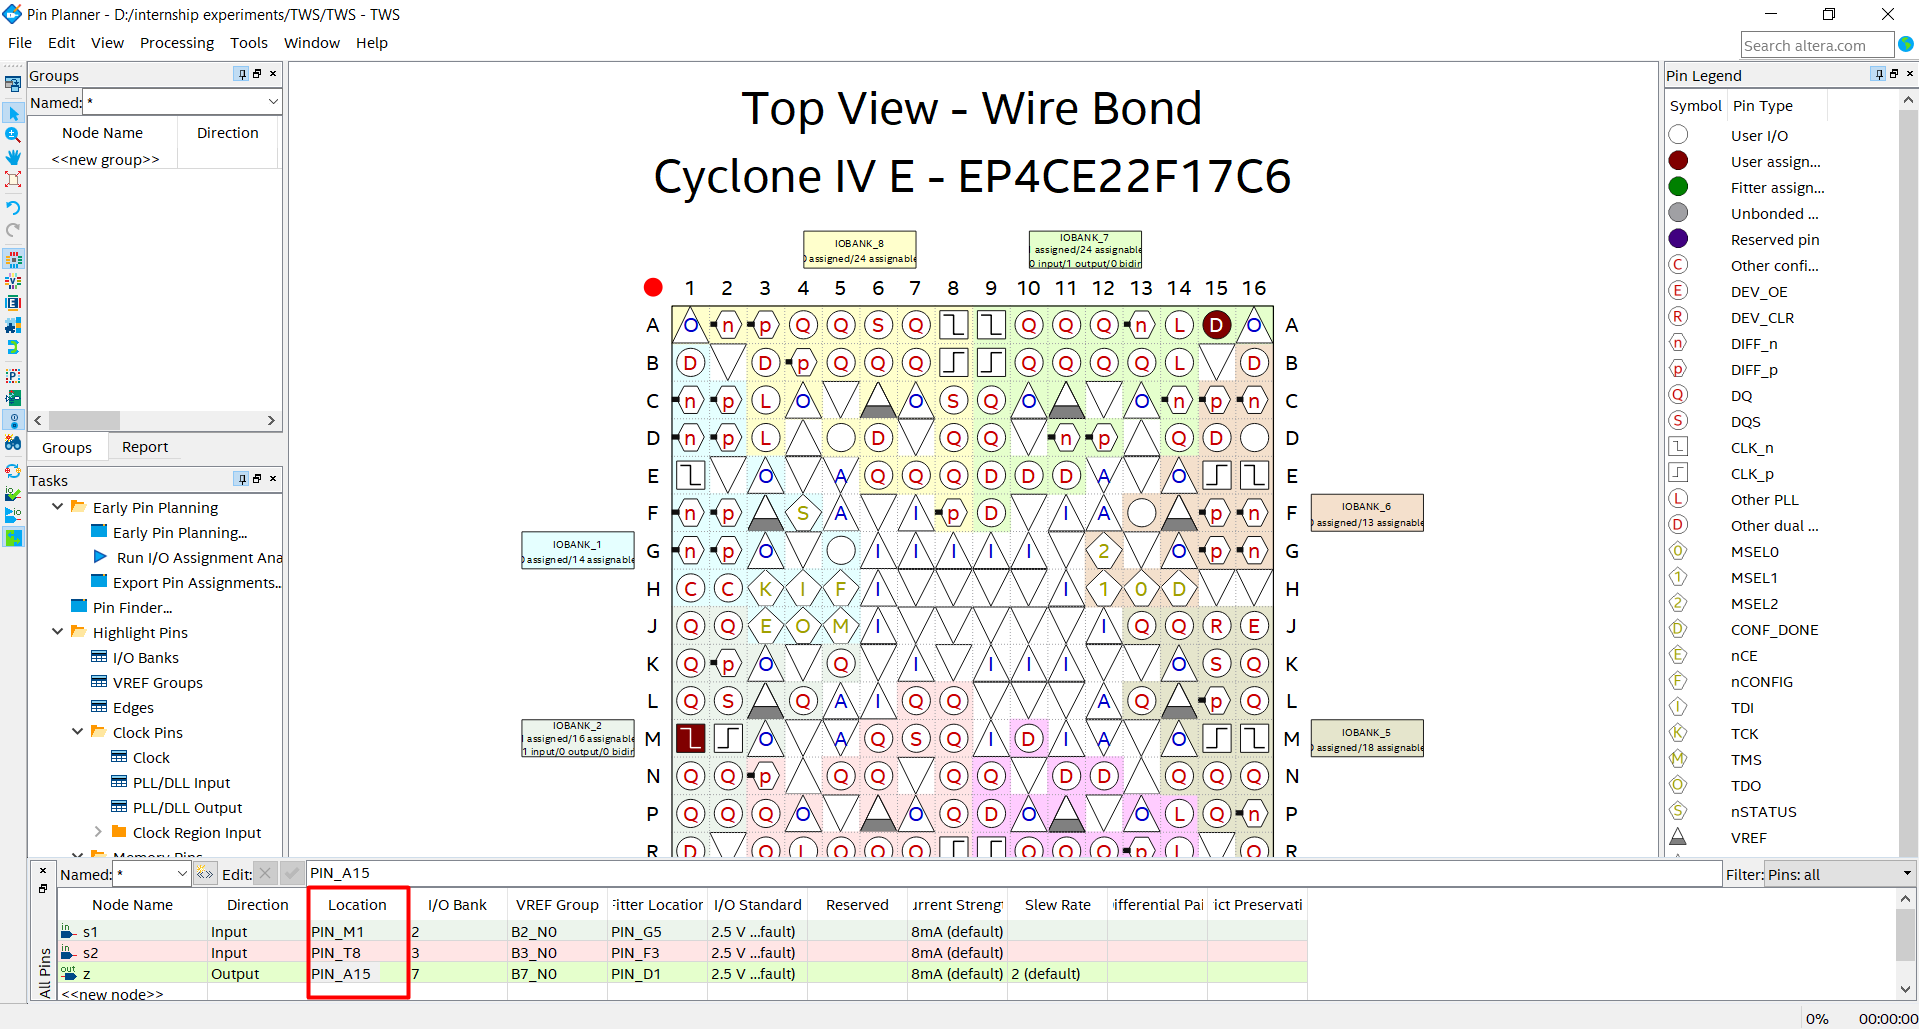
\includegraphics[scale=0.35 ]{TWSPLAN2.png}
    \end{figure}

    
    \item Go to \textbf{'Processing'$\rightarrow$ 'Start I/O Assignment Analysis'}.
        \begin{figure}[H]
             \centering
            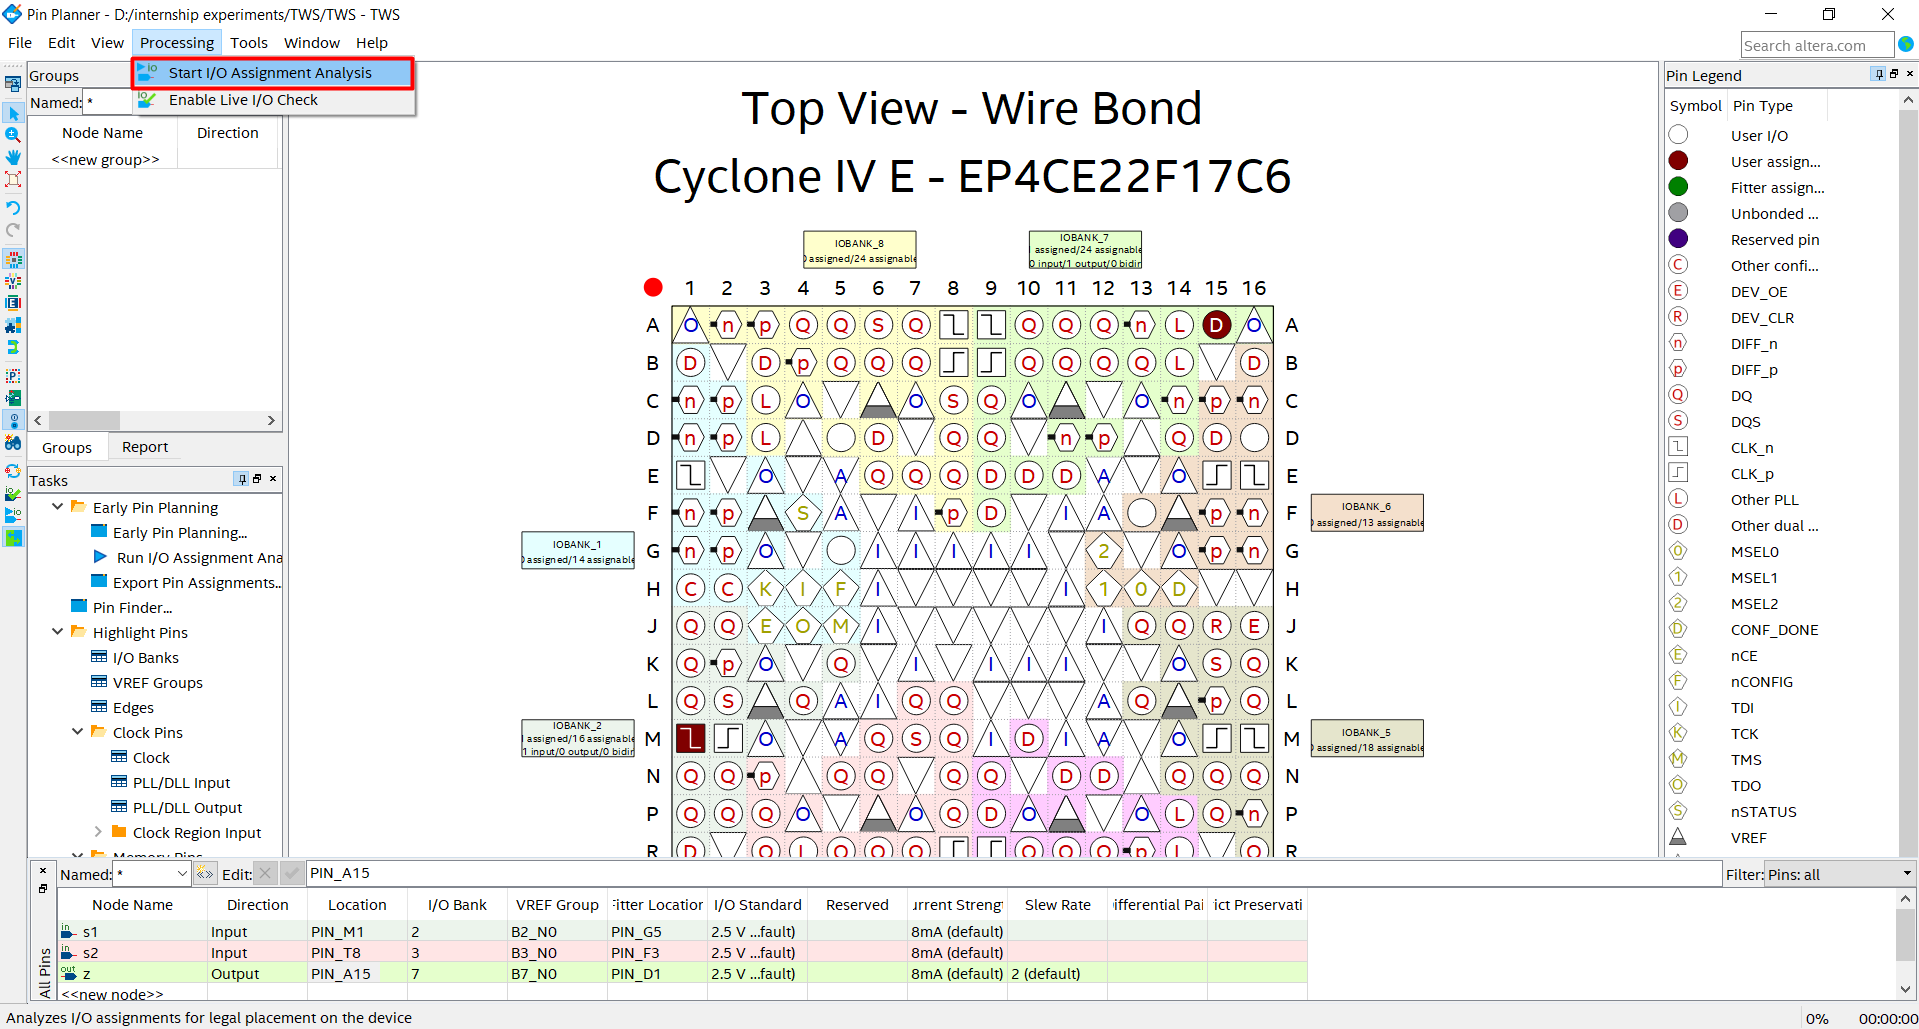
\includegraphics[scale=0.35 ]{TWSPLAN3.png}
         \end{figure}
\end{enumerate}
\newpage
 \section{Downloading the code to DE0 Nano FPGA Board}
 Before starting, Make sure the board is powered ON and connected to the computer through an USB Cable
 
 \begin{enumerate}
     \item \textbf{'Compile'} the Project by double clicking on compile or the \textbf{'Play'} button. This creates an SRAM object file(.SOF file). This file is used to program the Device
     \begin{figure}[H]
         \centering
         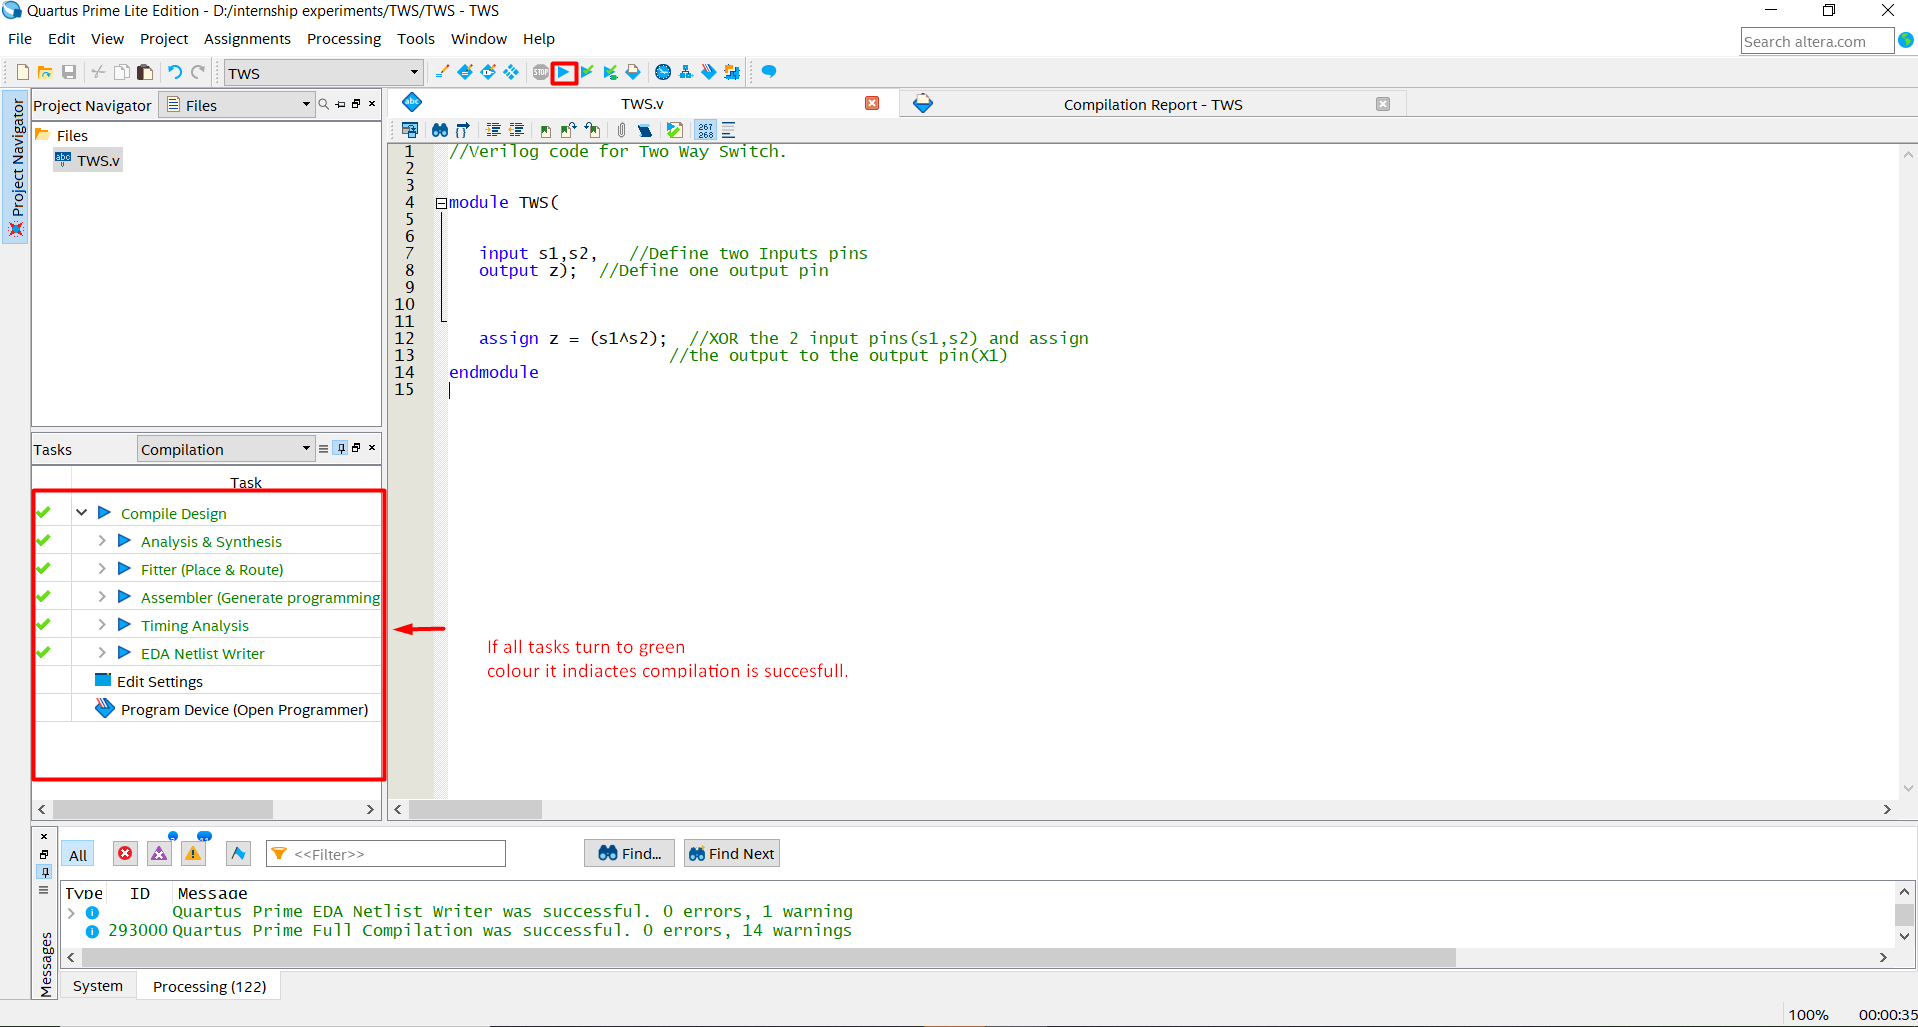
\includegraphics[scale=0.32]{twsd1.png}
     \end{figure}
     
     \item Open the programmer by going to \textbf{'Tools'$\rightarrow$ 'Programmer'}
     \begin{figure}[H]
         \centering
         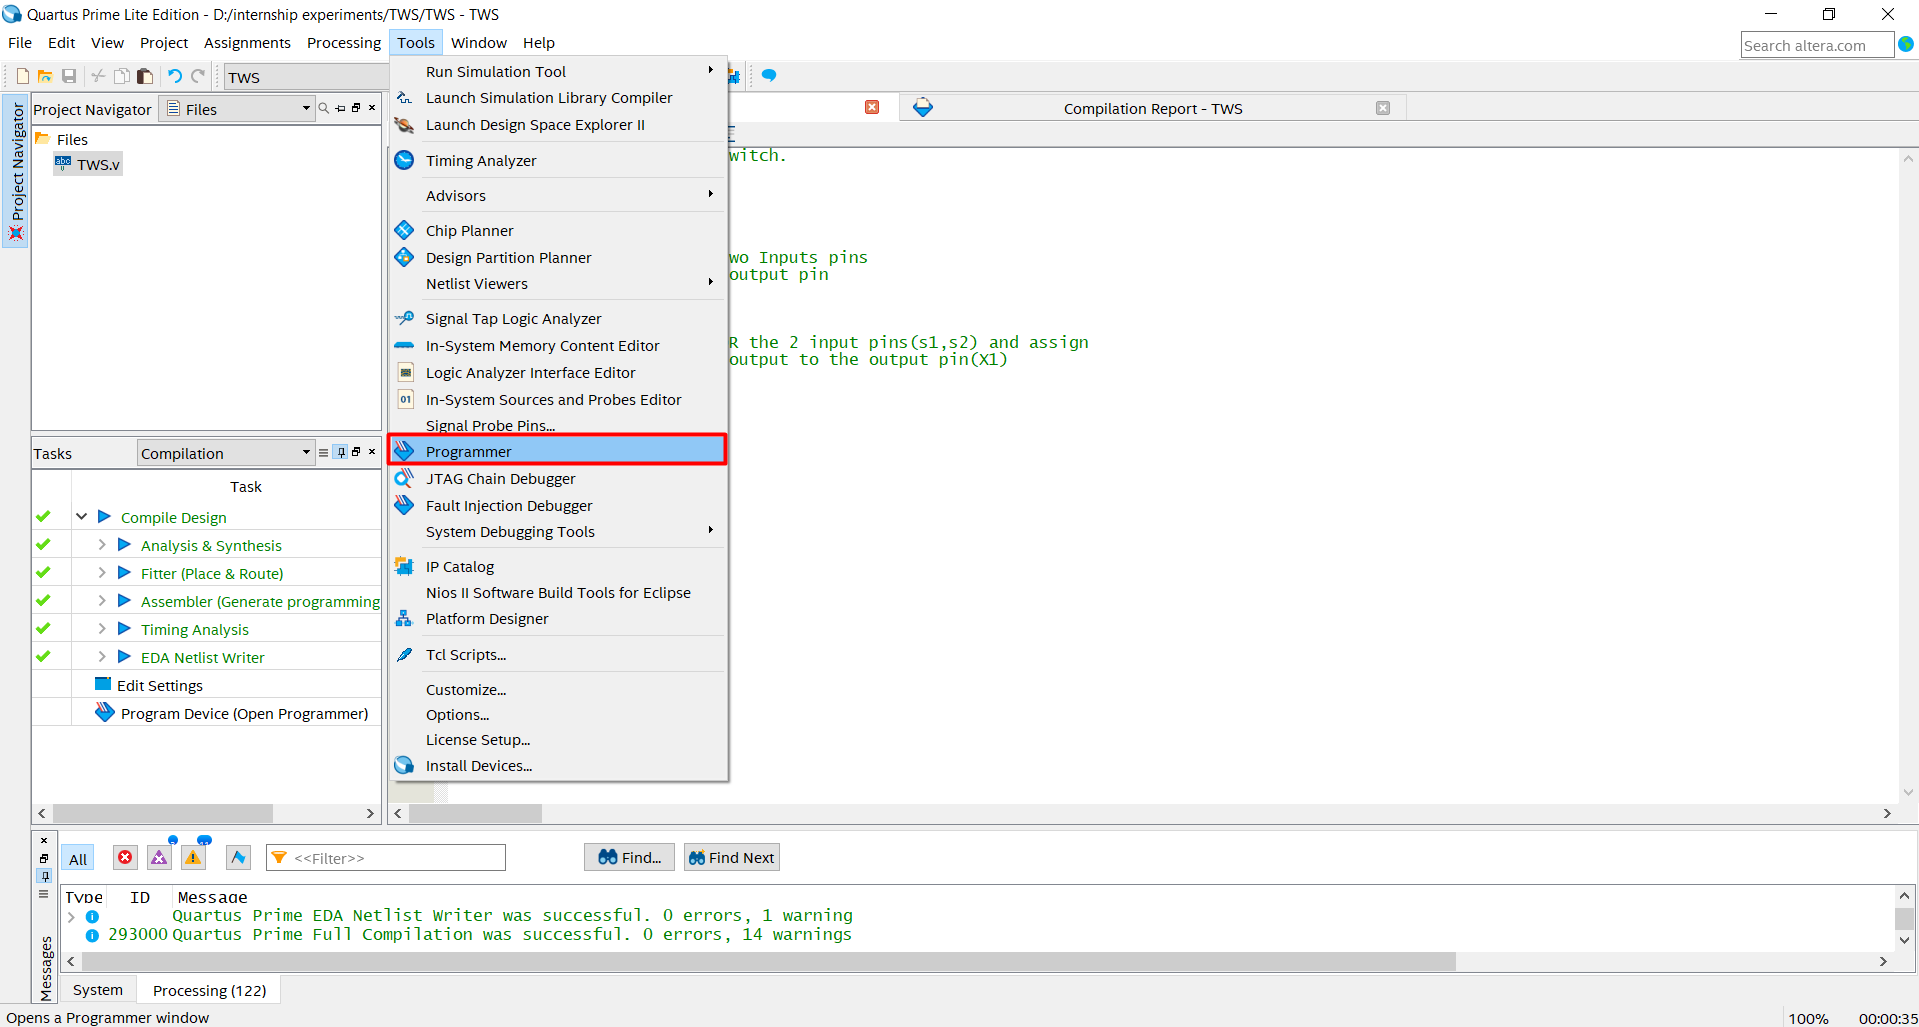
\includegraphics[scale=0.32]{twsd2.png}
     \end{figure}
     \newpage
     \item Click on \textbf{'Hardware Setup'}. The Device required must be listed under "Currently available hardware". If not, check if the device drivers are correctly installed. Choose the hardware from the dropdown menu
     \begin{figure}[H]
         \centering
         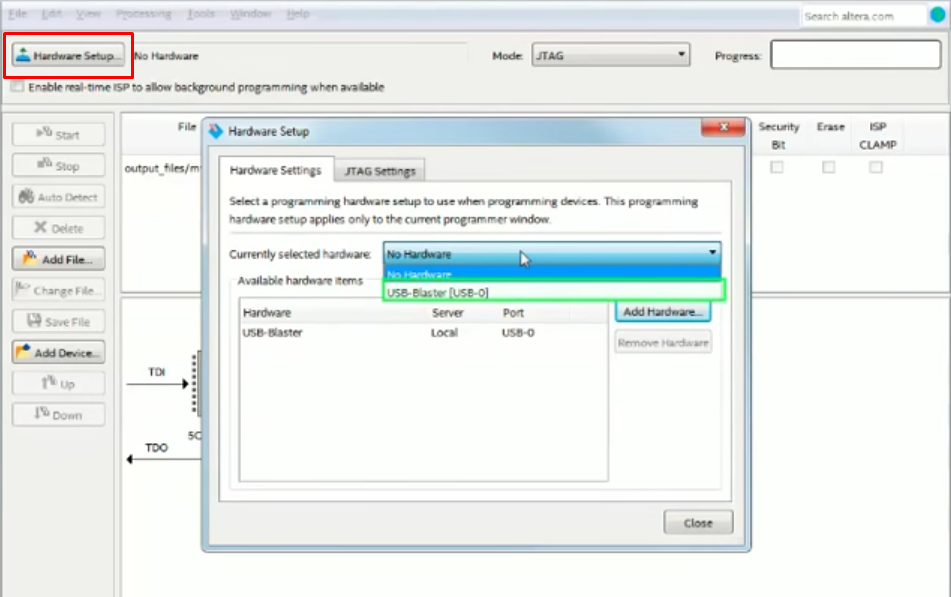
\includegraphics[scale=0.4]{downloading to board/3.png}
     \end{figure}
     
     \item In case you didn't find the '\textbf{USB\-BLASTER}' option. Click on '\textbf{AUTO DETECT}' to see if the program can find the device. If it still couldn't find it, check if the device drivers are correctly installed. Refer your device's manual for more information.\newline
     \textbf{Note:}The '\textbf{AUTO DETECT}' Button will be highlighted when you connect your board to your computer
      \begin{figure}[H]
         \centering
         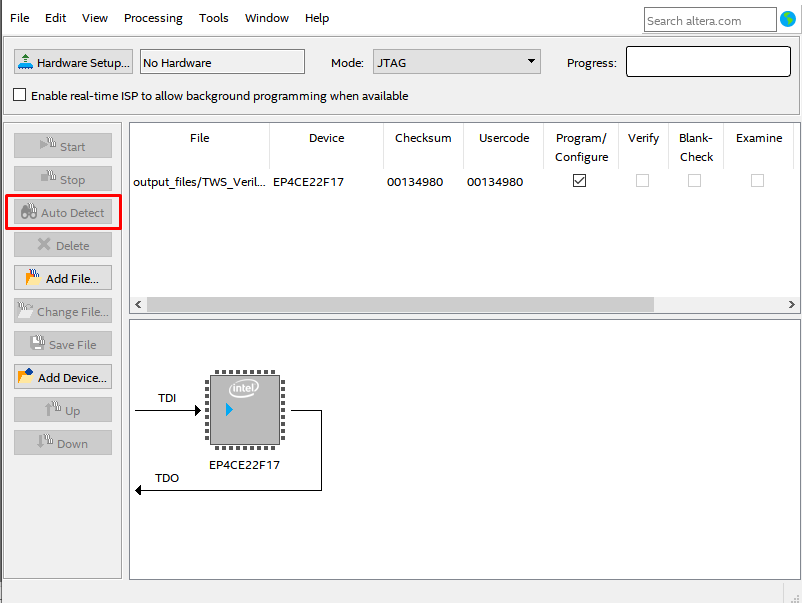
\includegraphics[scale=0.45]{autodetect_hardware.png}
     \end{figure}
     
     \item If the file is not listed, it can be manually added by clicking on add file. The .SOF file can be found the output directory inside the project directory 
     \begin{figure}[H]
         \centering
         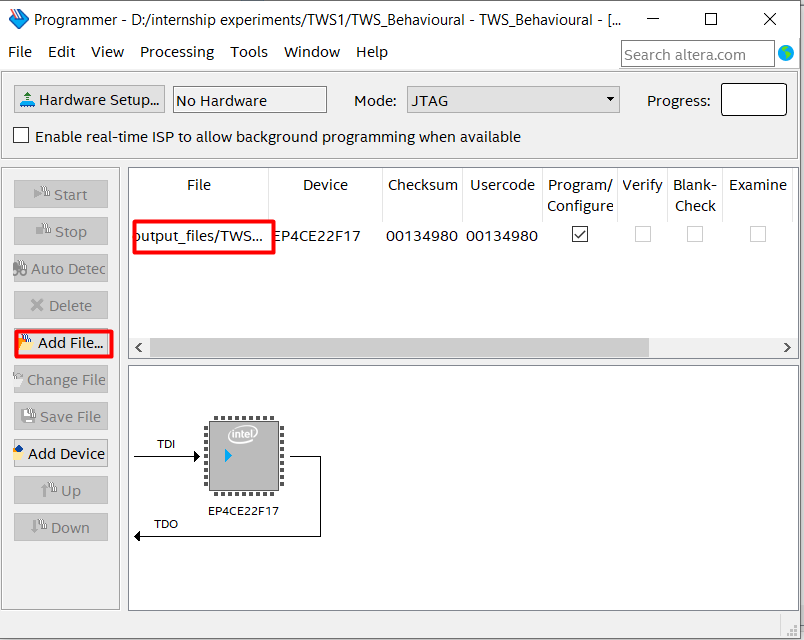
\includegraphics[height=8cm,keepaspectratio]{download1.png}
     \end{figure}
     \item Make sure the \textbf{'Program/Configure'} checkbox is ticked
     \begin{figure}[H]
         \centering
         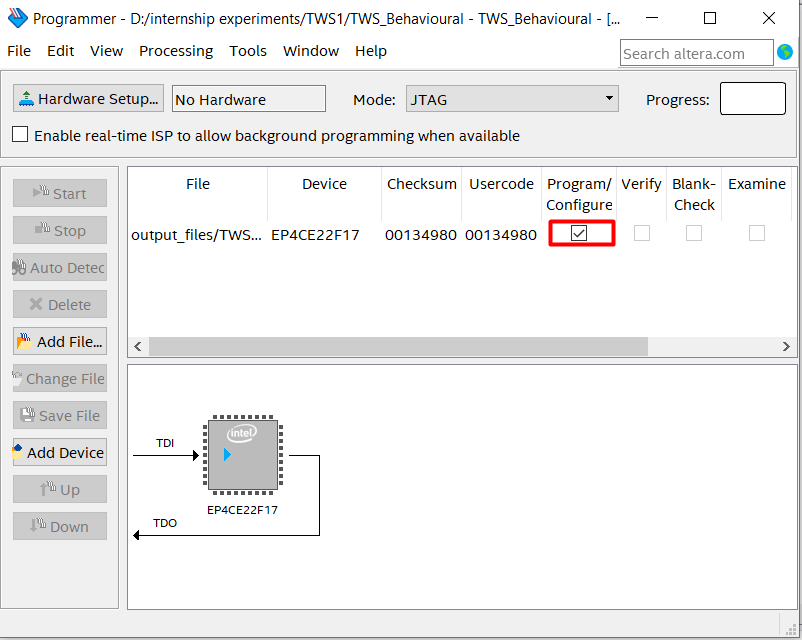
\includegraphics[height=8cm,keepaspectratio]{download2.png}
     \end{figure}
     \item When ready, click on \textbf{'Start'}to start the programming process .\textbf{'Start'} button will be enabled when the 'DEO NANO' board is connected to USB port of your device. 
     \begin{figure}[H]
         \centering
         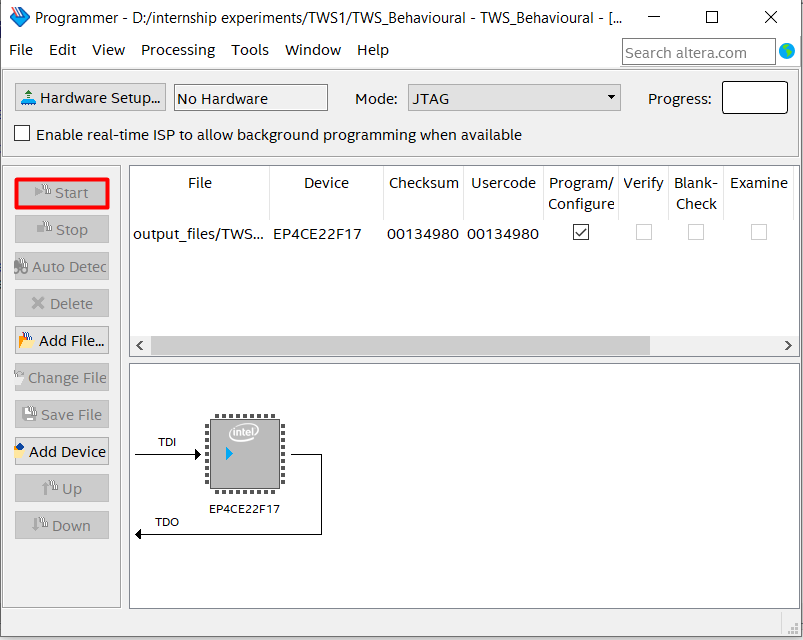
\includegraphics[height=7cm,keepaspectratio]{download3.png}
     \end{figure}
     
 \end{enumerate}

\newpage
\section{Implementing on Modelsim }
The TestBench shown here is a Verilog TestBench. For more detailed procedure on using ModelSim, Refer '\textbf{Quick Start Guide to Quartus and ModelSim Software}' Document
 \begin{enumerate}
     \item Create a \textbf{NEW} Verilog file in Quartus Prime.Type in the TestBench code provided in this document and \textbf{SAVE} the file with the same name as the module name
    \begin{figure}[H]
        \centering
    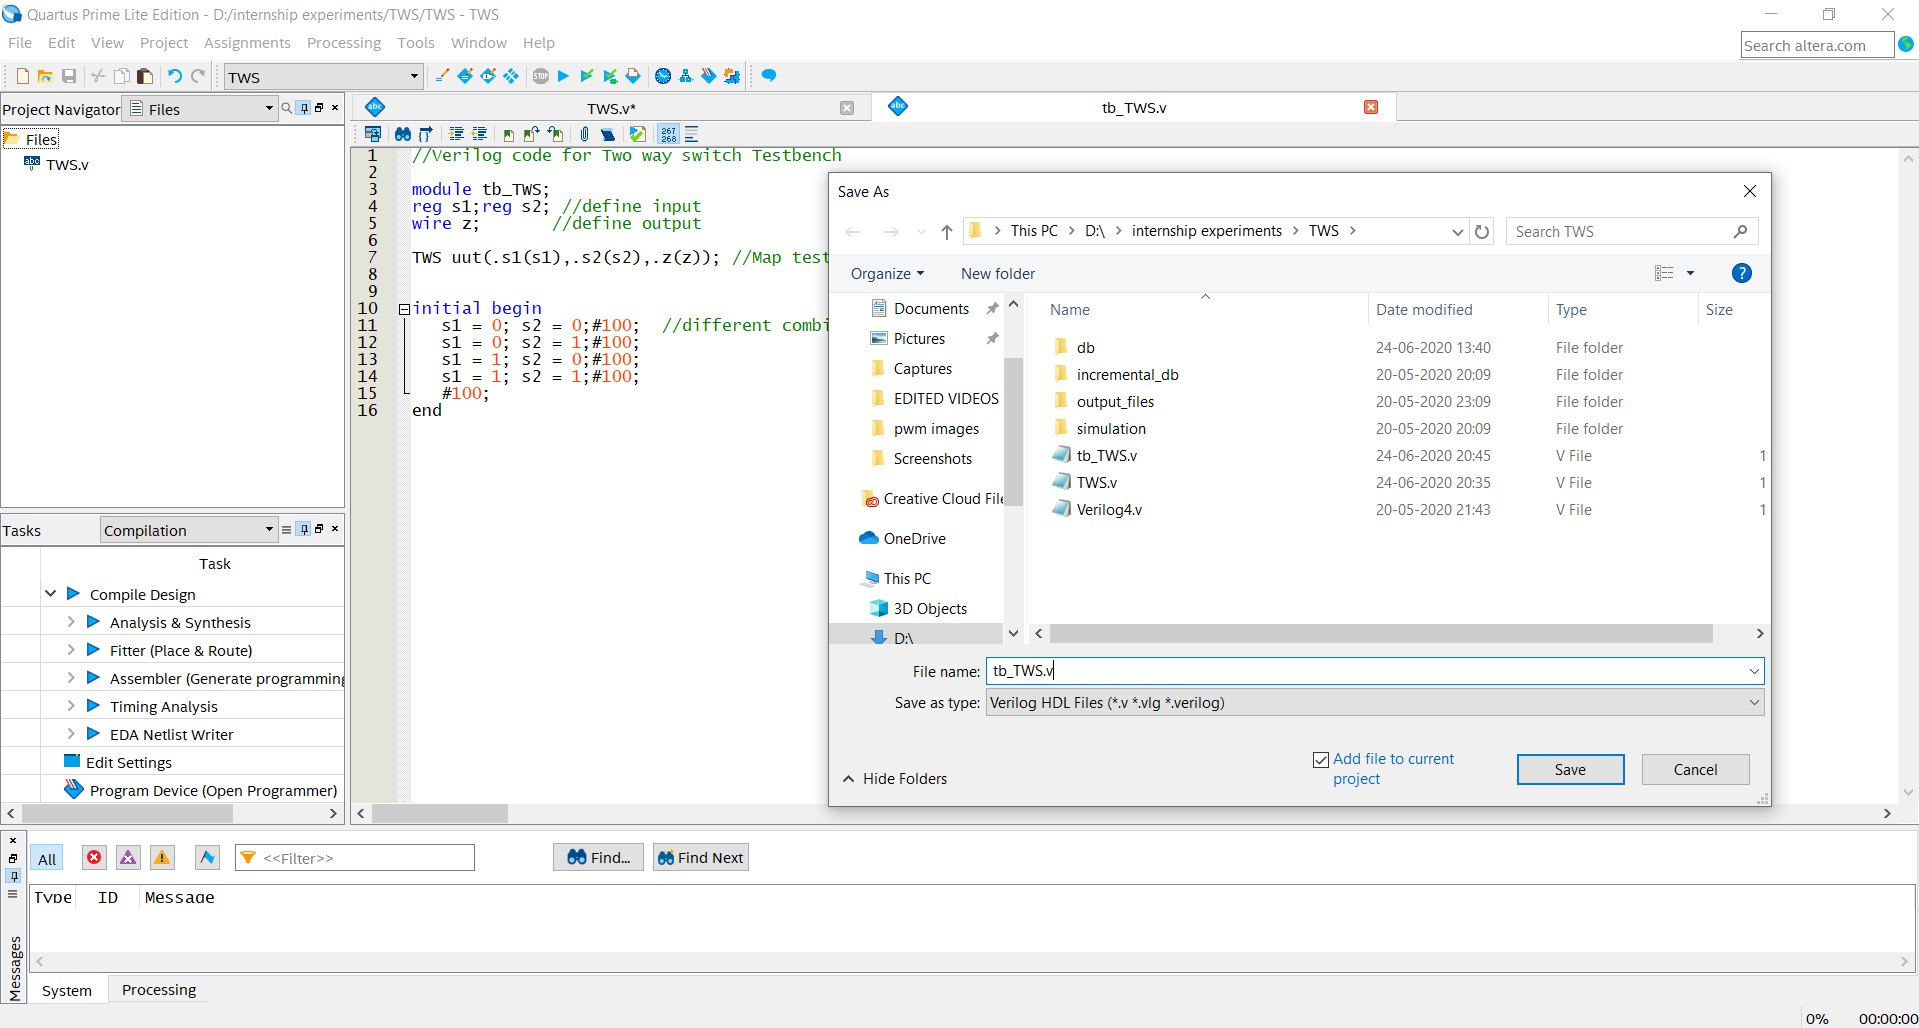
\includegraphics[width=14cm,keepaspectratio]{twstbadd.png}
    \end{figure}
    \newpage
   
    \vspace{5mm}
    \\
    \item Go to \textbf{'Assignments'$\rightarrow$'Settings'}.
    \begin{figure}[H]
        \centering
    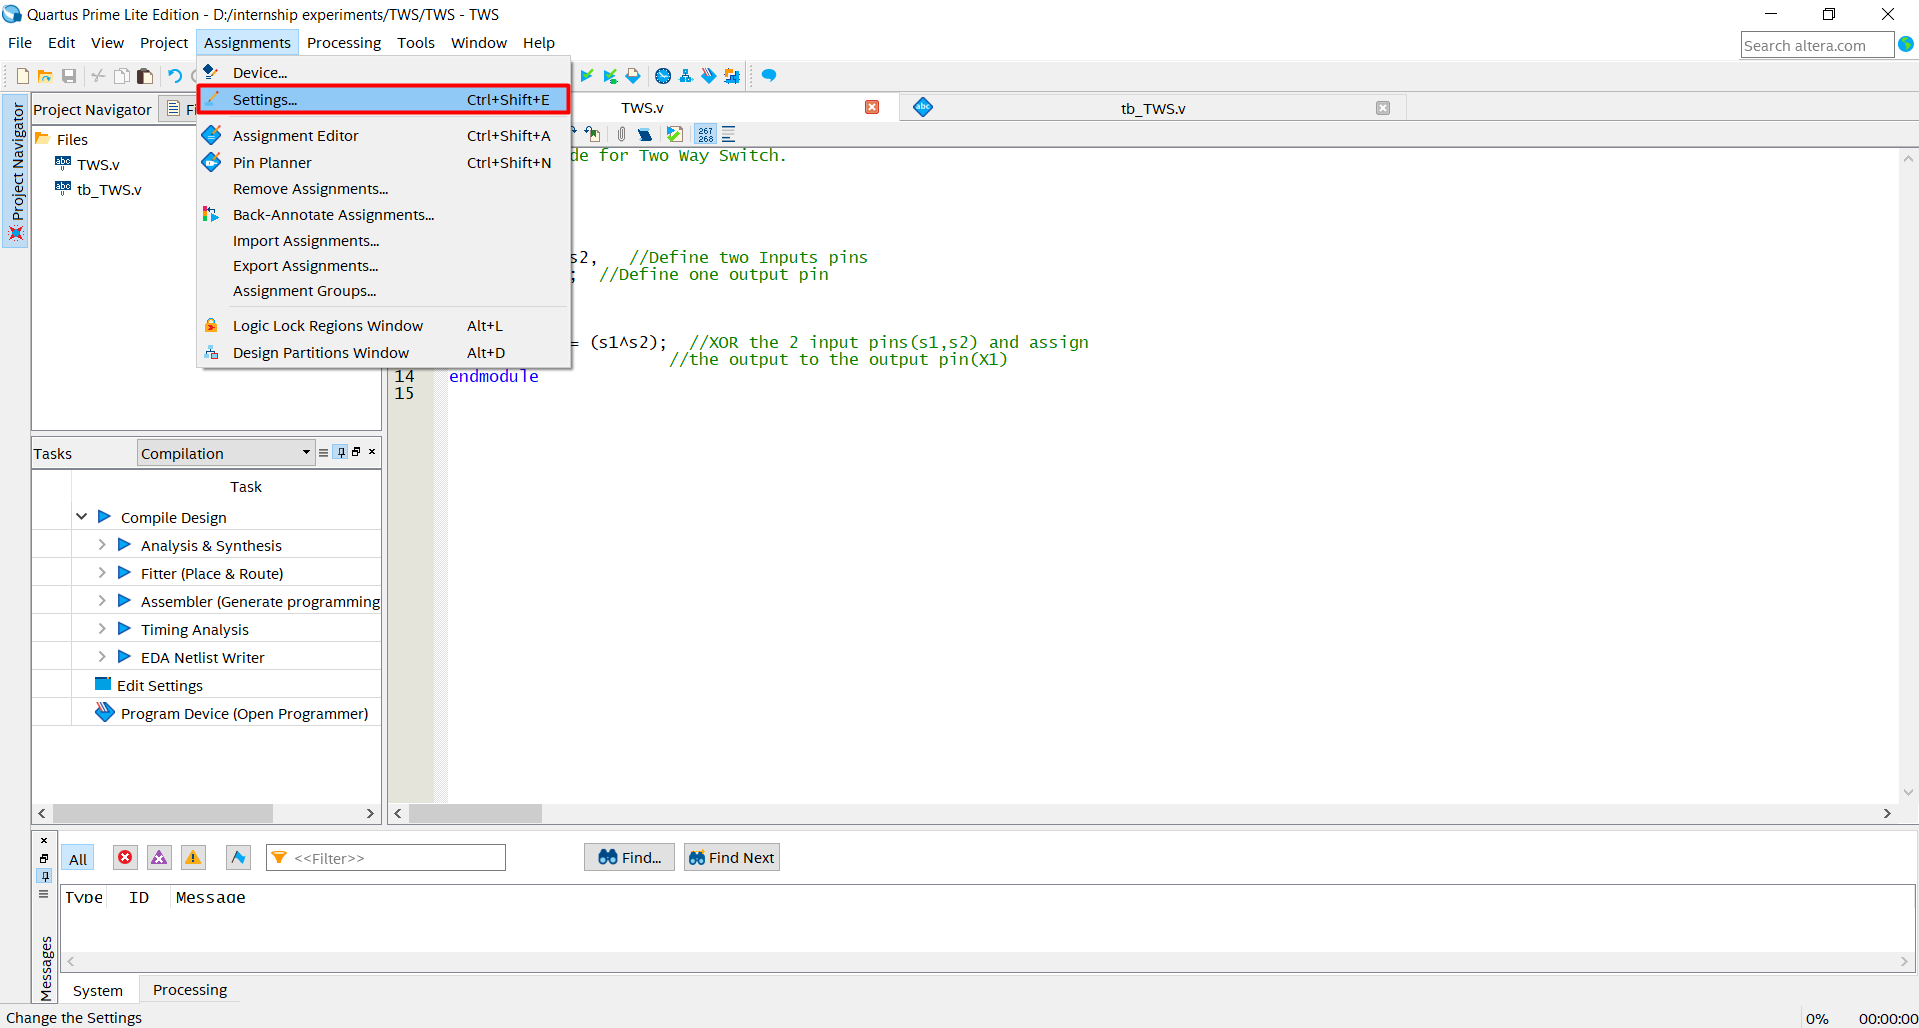
\includegraphics[width=14cm,keepaspectratio]{tws4.png}
    \end{figure}
    \item Navigate to \textbf{ 'Simulation'} under \textbf{'EDA Tool Settings'}.Set the language as Verilog HDL. Select \textbf{'Compile Test Bench'} and then click on \textbf{'Test Benches'}.
    \begin{figure}[H]
        \centering
    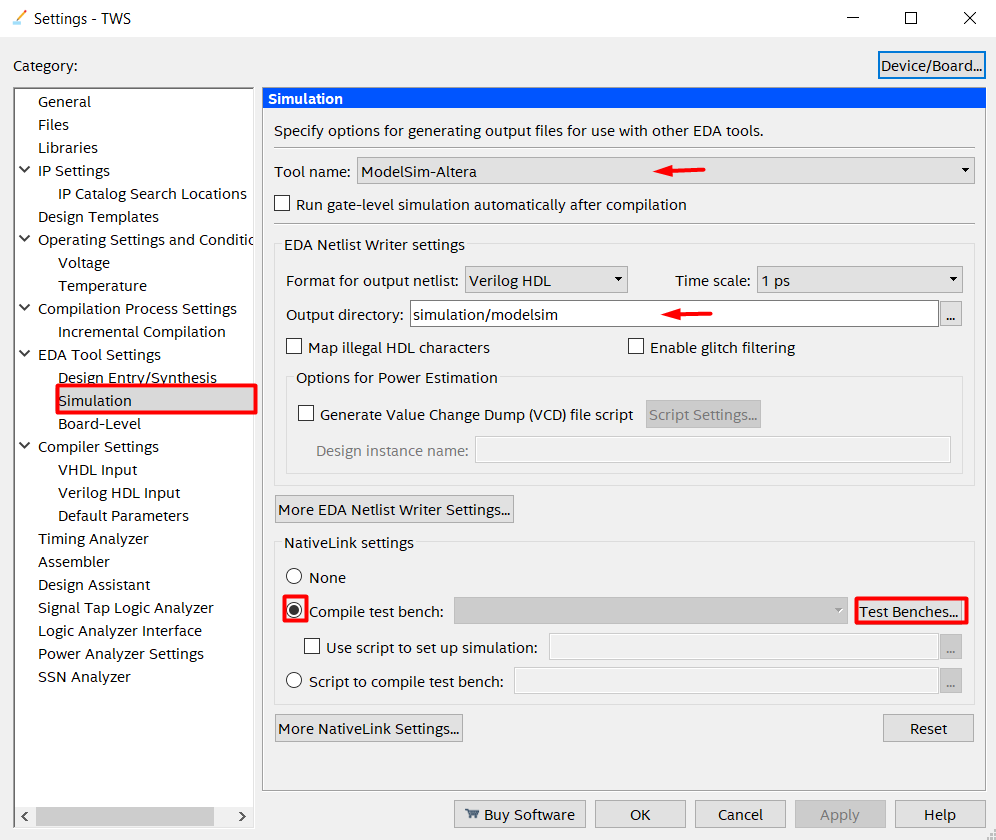
\includegraphics[width=10cm,keepaspectratio]{tws5.png}
    \end{figure}
    \newpage
    \item Click on \textbf{'New'}, this opens another dialogue box.
    \begin{figure}[H]
        \centering
    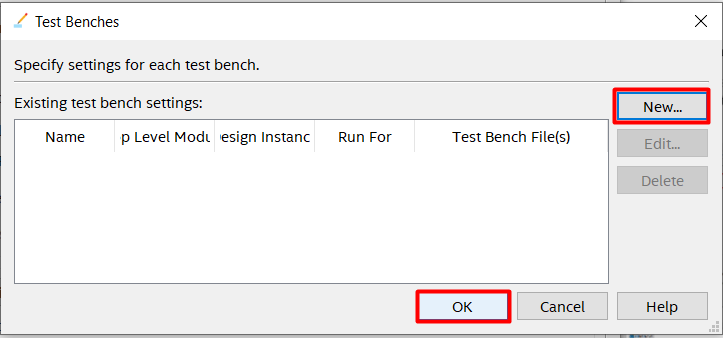
\includegraphics[width=14cm,keepaspectratio]{tws6.png}
    \end{figure}
    
    \item Now type in the testbench name(In this design , its \textbf{tb\_TWS}). Now click on the highlighted browse button.Find the testbench file(it can be found in the project directory) and click on \textbf{'Open'}. Now click on \textbf{'Add'},then \textbf{'OK'}.
            \begin{figure}[H]
        \centering
    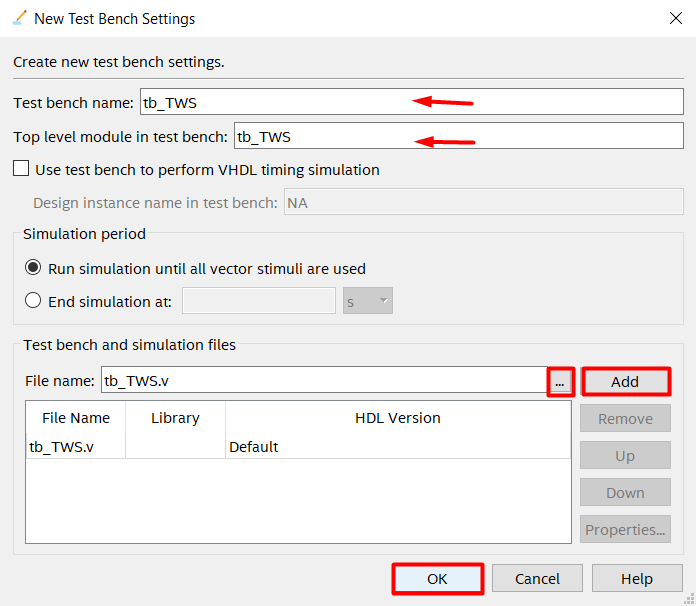
\includegraphics[scale=0.73]{tws7.png}
    \end{figure}
    
 \end{enumerate}
 \newpage
 \noindent \textbf{Functional Simulation using NativeLink Feature}
    \begin{enumerate}
        
        \item  Go to menu \textbf{'Processing'} $\rightarrow$ \textbf{'Start'} $\rightarrow$ \textbf{'Start Analysis \& Elaboration'}.After this click on \textbf{'Start Analysis \& Synthesis '}on the same drop box. 
            \begin{figure}[H]
                \centering
                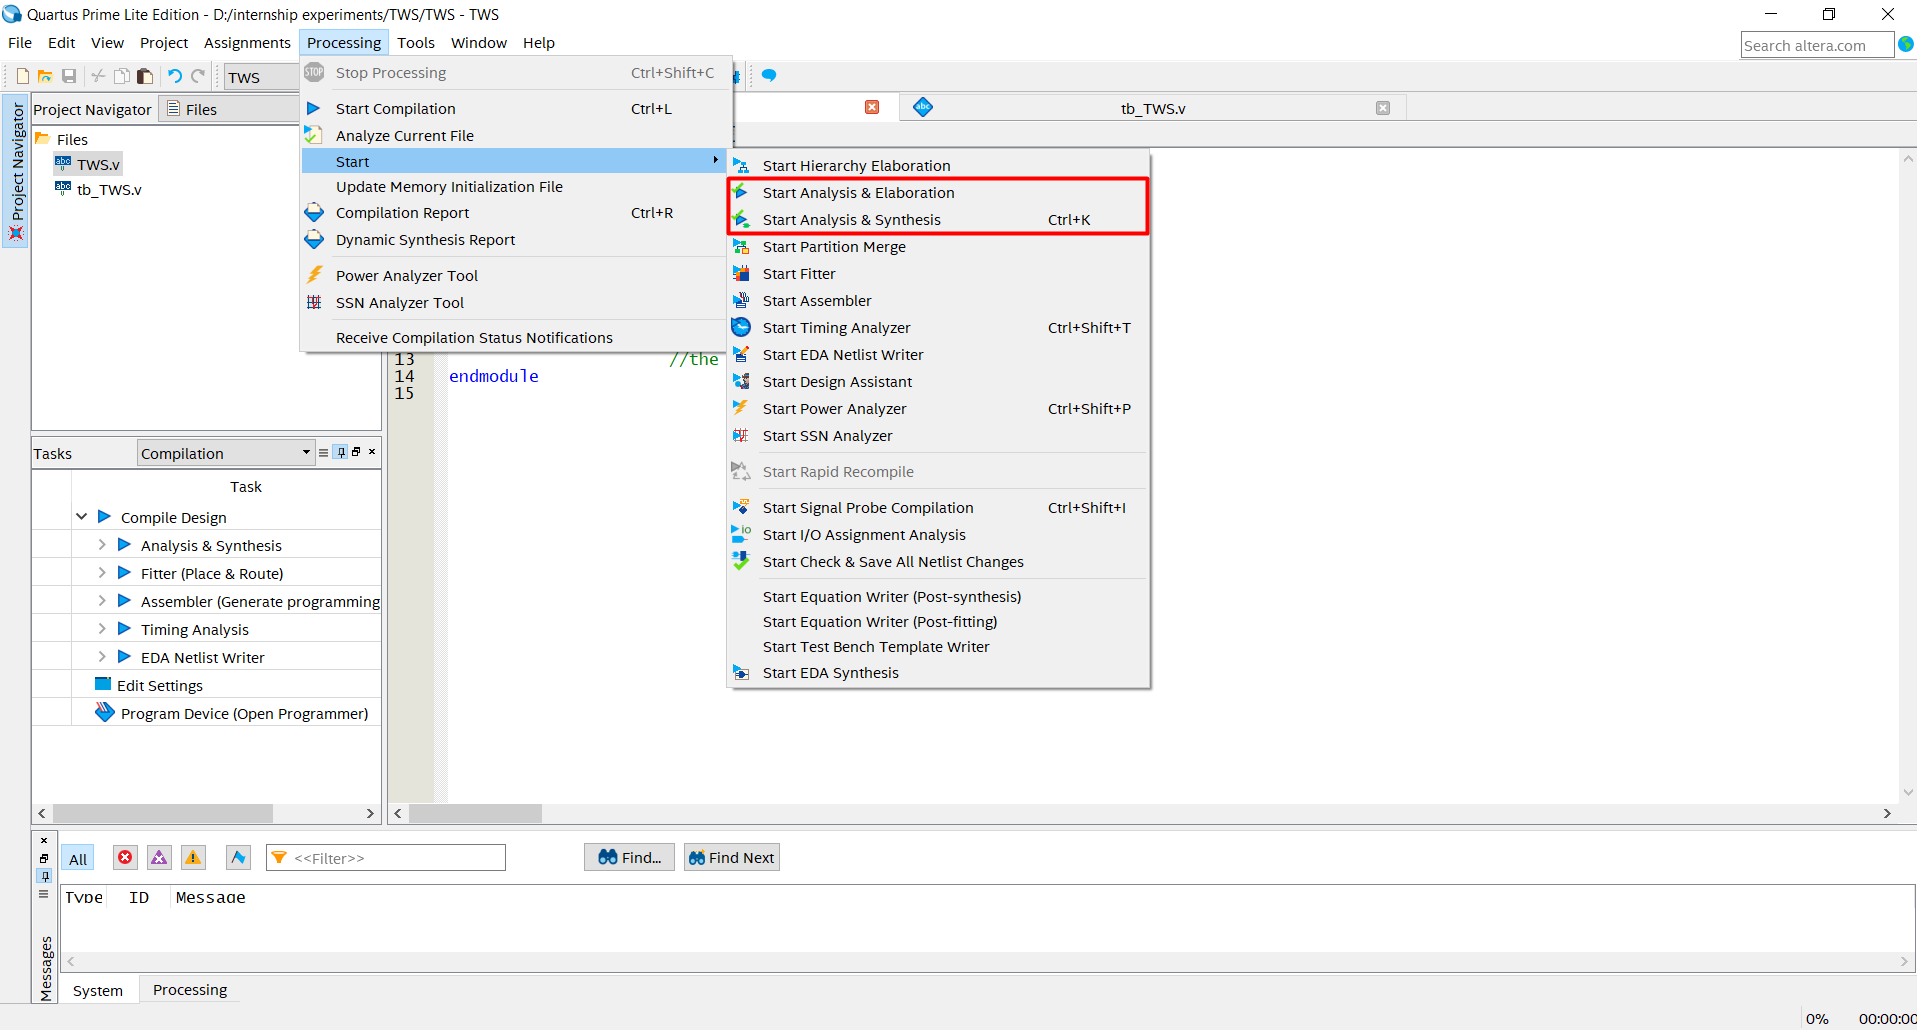
\includegraphics[width=14cm,keepaspectratio]{tws8.png}
            \end{figure}
    
        
        \item Go to menu \textbf{'Tools' $\rightarrow$ 'Run Simulation Tool' $\rightarrow$
         “RTL Simulation”} to automatically run the EDA simulator(ModelSim-Altera) and to compile all necessary design files.
            \begin{figure}[H]
                \centering
                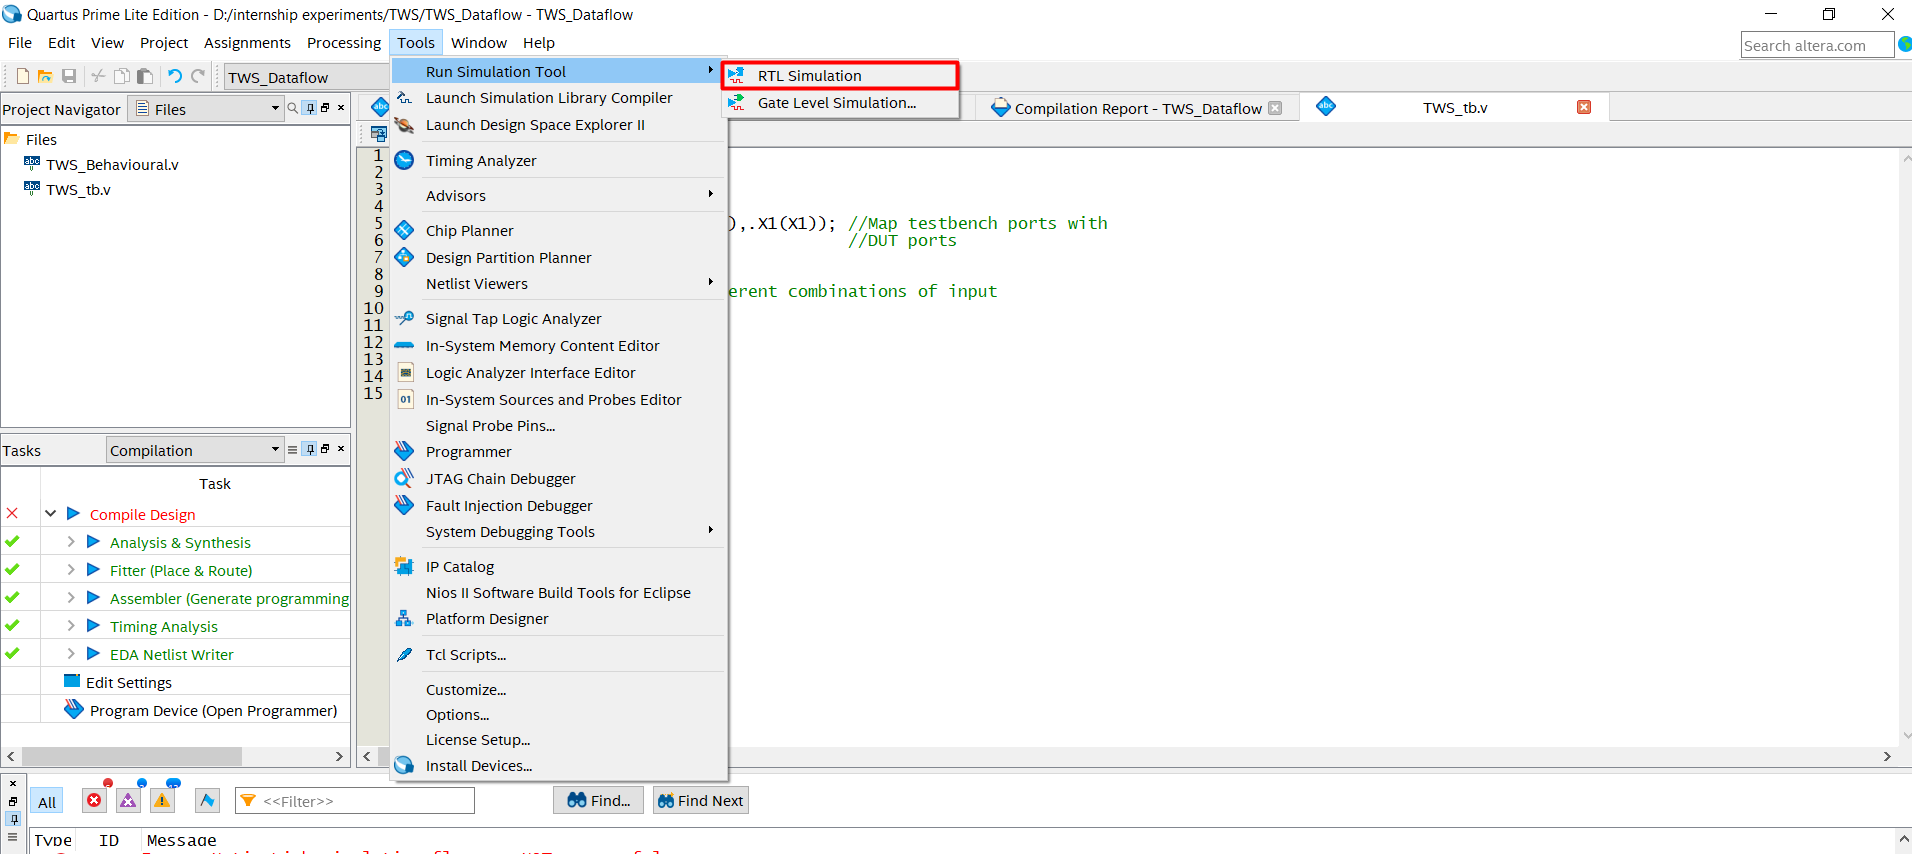
\includegraphics[width=14cm,keepaspectratio]{simu5.png}
            \end{figure}
    \newpage
        \item Finally ModelSim-Altera tool opens up with simulated waveform. click on \textbf{'Run all'} icon on the tool box to display the waveform.
            \begin{figure}[H]
                \centering
                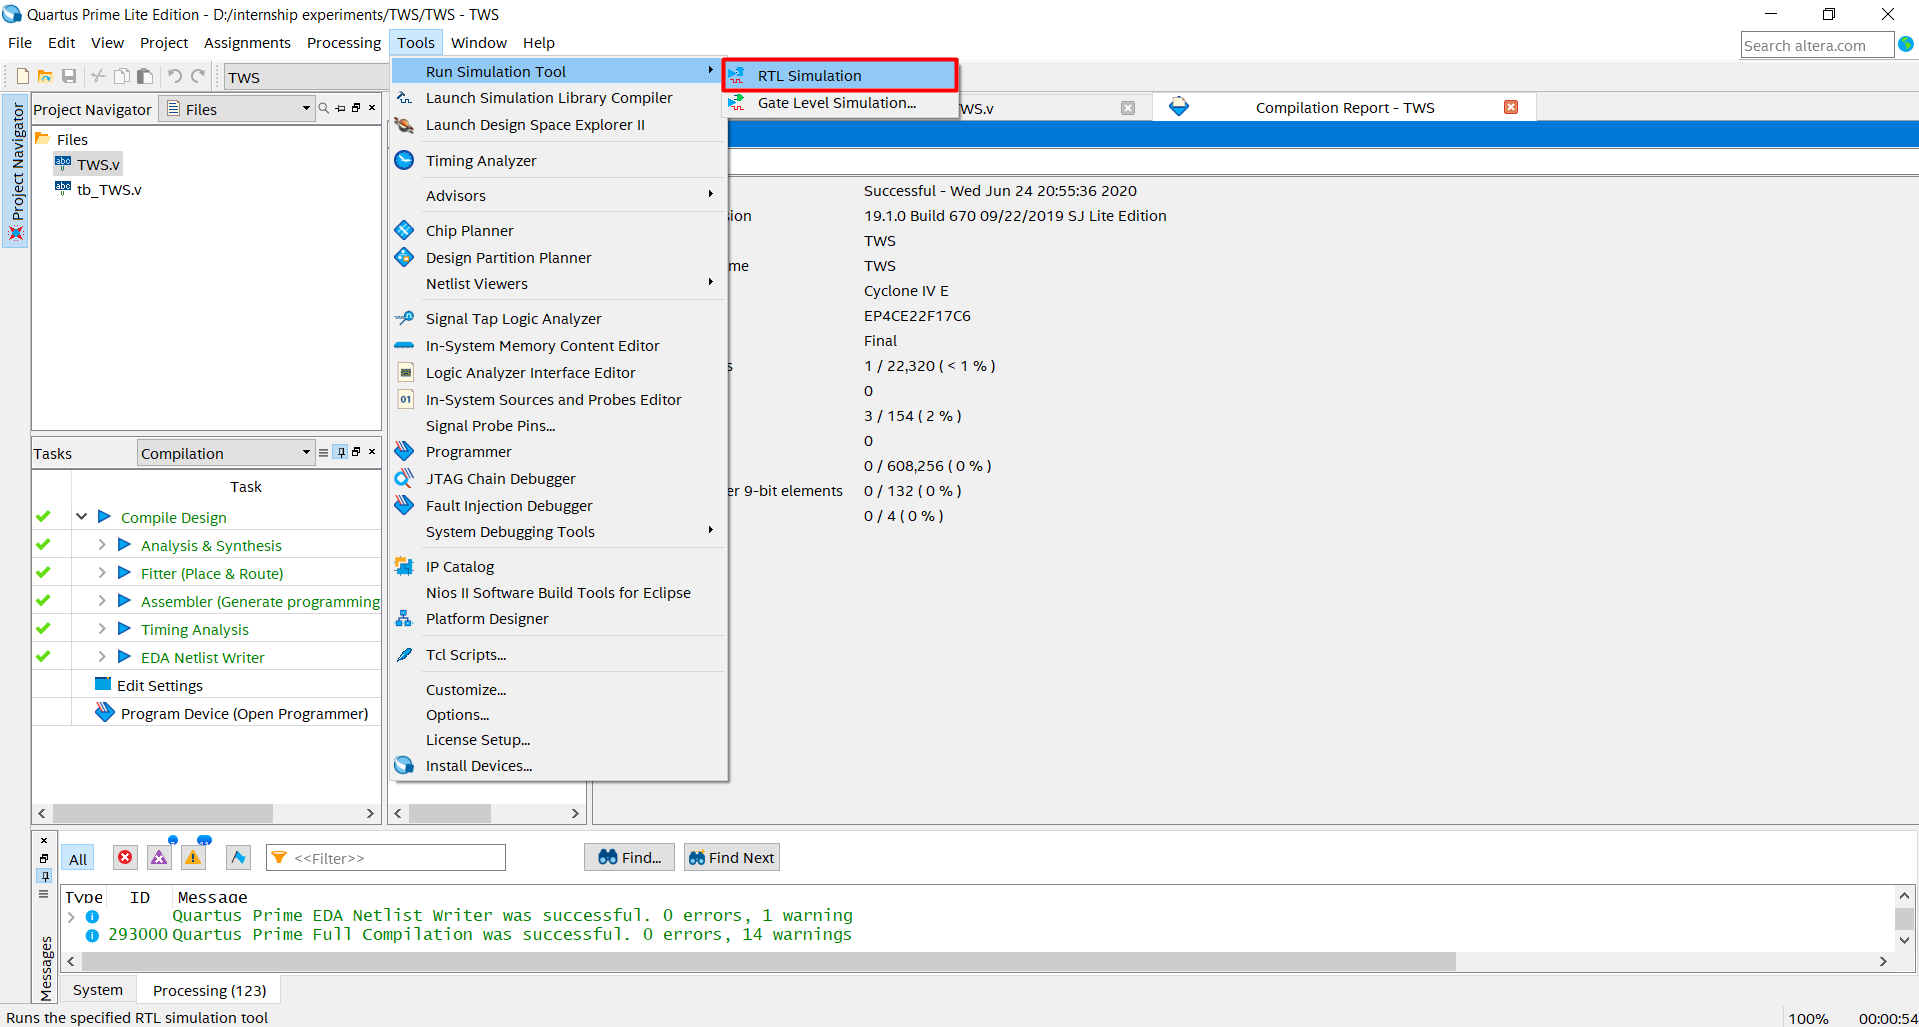
\includegraphics[width=14cm,keepaspectratio]{tws9.png}
            \end{figure}
  
        
    \end{enumerate}
 \newpage
 
 
\section{Testing the Design}
What you see below is the simulation waveform obtained in ModelSim. Consider the Verilog design, from the waveform, we can see that when '\textbf{s1 = 0}' and '\textbf{s2 = 0}' the output '\textbf{z = 0}'. When '\textbf{s1 = 0}' and '\textbf{s2 = 1}' the output '\textbf{z = 1}'. When '\textbf{s1 = 1}' and '\textbf{s2 = 0}' the output '\textbf{z = 1}'.When '\textbf{s1 = 1}' and '\textbf{s2 = 1}' the output '\textbf{z = 0}'. This is the logic of a XOR Gate. The same can be observed in the VHDL design.Hence the design has been verified
\subsection{Simulation waveform of the Verilog Design}

\begin{figure}[H]
    \centering
    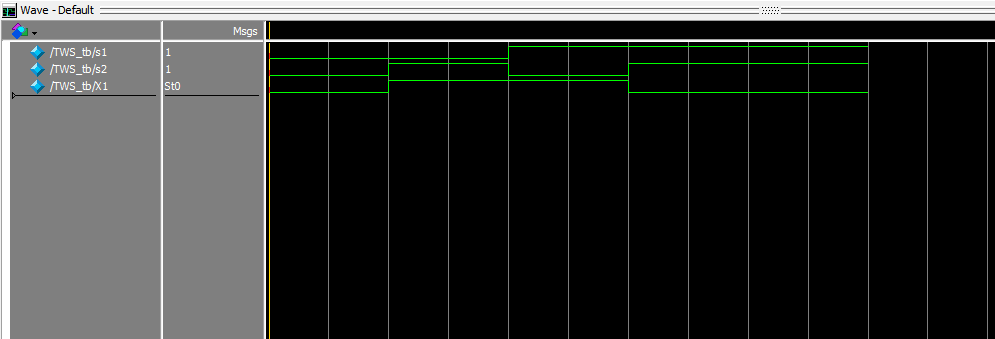
\includegraphics[width = 14cm,keepaspectratio]{simulation_waveform_verilog/Simulation_waveform.png}
\end{figure}

\subsection{Simulation waveform of the VHDL Design}

\begin{figure}[H]
    \centering
    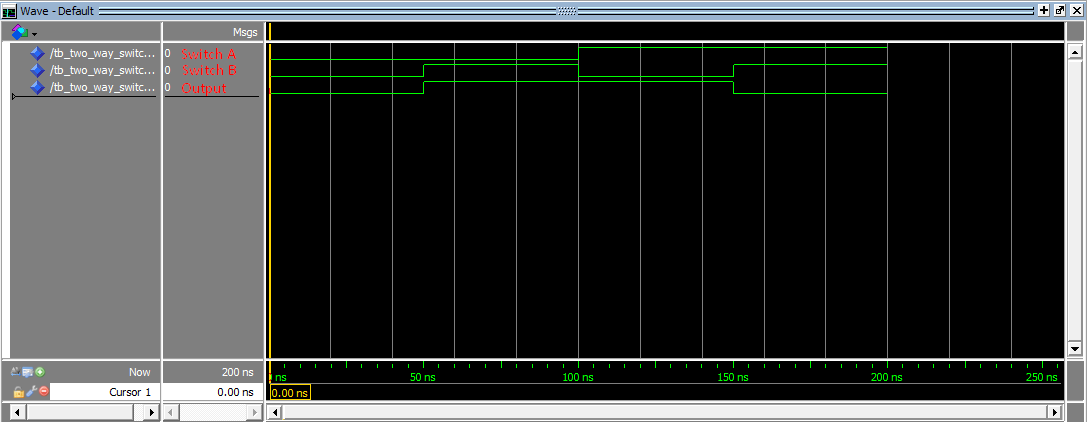
\includegraphics[width = 14cm,keepaspectratio]{op.png}
\end{figure}





\end{document}

